\chapter{Software Detail Design}
\label{chap:4}

In this chapter, the software design aspects of this project are discussed in
detail.

This chapter is divided up into four sections, with each section explaining what
the program being discussed is responsible for, what third party programs it
uses and how it interacts with the rest of the system. 

These four sections are:

\begin{enumerate}
  \item The security scheme used.
  \item The web server that was created.
  \item The vending machine's control program.
  \item The Android app that was created.
\end{enumerate}

\section{Security Scheme}
\label{sec:security-code-scheme}

In addition to the asymmetric encryption used on all data transfer to and from
the server to its clients, two more layers of security were added to prevent
repeated use of the same code and to make it harder for hackers to crack the
encryption key.

\subsection{Random Character String}

The product code transmitted to the server is embedded inside a
random 16-character string of hex values, i.e. numbers from 1 to 9 or characters
from A to F. The product code is a 4 character hex string, but this is saved on
the database and can therefore not be random. 

This is done to prevent any would-be
hackers from realising that they have cracked the system's encryption. In other
words, if the hackers have cracked the encryption, they will still see 16
random hex characters and think that the encryption is still intact.

\subsection{Challenge and Response Code}

The second layer of security added is a challenge/response system. Such a system
works by having party A generate a challenge (this can be a string or a number).
Party B then takes this challenge and puts it through a previously agreed-upon
process, e.g. makes the letters capital or adds the numbers together. This
is the response. Party B then sends the back the response to party A, which then
checks to see if its a valid response to party A's original challenge.

In the case of the vending machine, a 16 character hex string is being
generated. It was decided to use 4 characters of this random string as the
vending machine's challenge. After receiving this challenge, the server then
takes out the agreed-upon 4 characters and adds it to the server's response
code. When the vending machine scans the customer's response QR Code, the
vending machine checks to see if the 4 character response was part of its
original code the vending machine generated.

This system is used to prevent customers from only buying one product and using
the same code again to get another product for free. Thus, the
challenge/response code system makes each code only valid for one transaction.

\section{Web Server Program Design}

The web server that was made for this project is based on the Django web framework for Python
(see Section \ref{sec:django} on page \pageref{sec:django} for some background information
on Django).
The Django server was then configured to run on top of an Apache web server located on an Amazon Web Service (AWS) Elastic
Compute Cloud (EC2) cloud computer instance (see Section \ref{sec:ec2} on page
\pageref{sec:ec2} for some background on EC2 and Section \ref{sec:apache} on page
\pageref{sec:apache} for some background on Apache).

The server is responsible for handling all the data and financial transactions that will take
place during the vending machine's operation. 

This section stipulates the design of the complete server and how the different components
interact with one another. 

\subsection{Django Server}

The Django server is responsible for all of the scripting and database work that the server
performs. The server is divided up into a total of six applications. Each of these is
responsible for either displaying a single web page or to handle data requests from the
Near Field Communication (NFC) Android app (see Section \ref{sec:nfc-android-app} on
page \pageref{sec:nfc-android-app} for more details on the Android app).

The website apps and their interactions with the real world and one another
are given in Figure \ref{fig:website-apps}.

\begin{figure}
 \centering 
 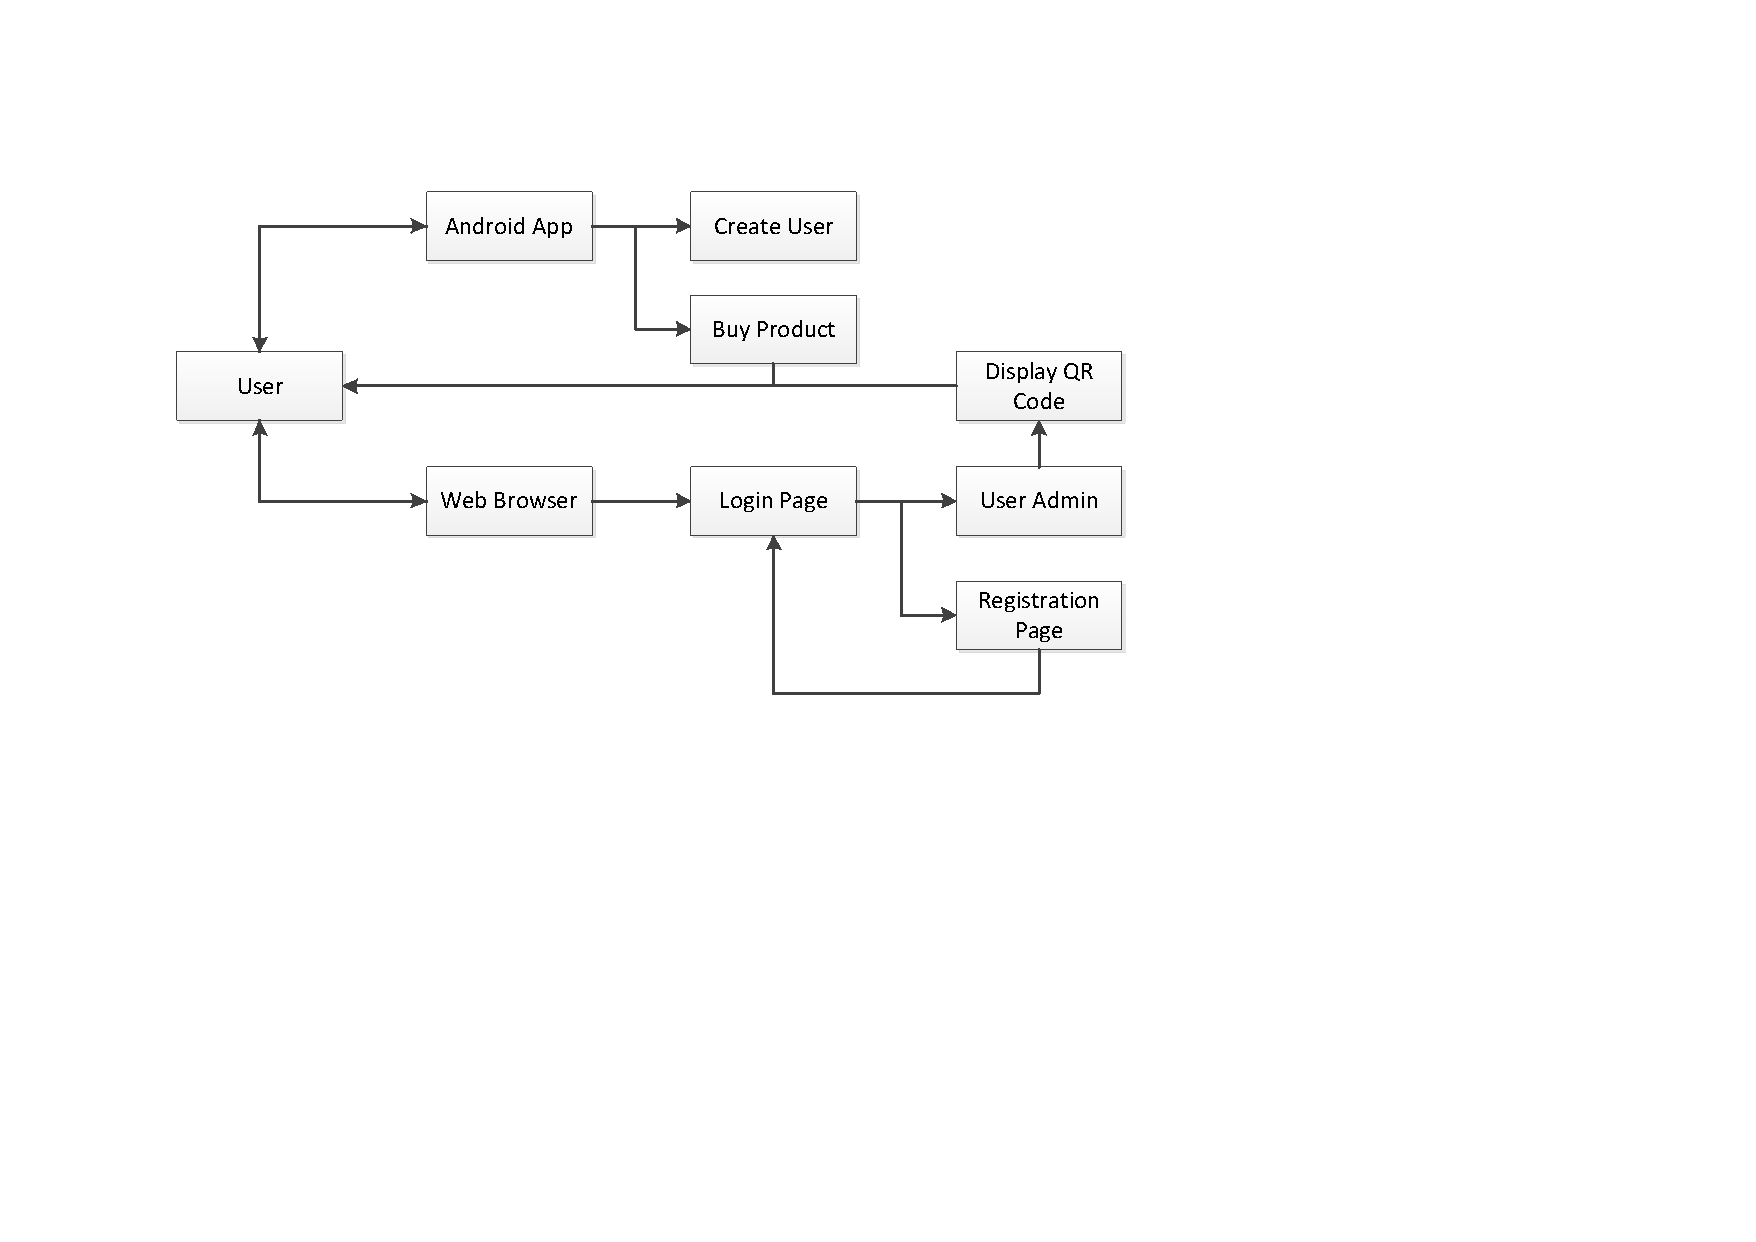
\includegraphics[clip=true, trim = 0 130 130 30,
 scale=0.7]{website_structure}
 \caption{The web server app structure}
 \label{fig:website-apps}
\end{figure}

\subsubsection{display\_qrcode}

This app forms the core of the Quick Response Code (QR Code) payment handling part of the
server. See Figure \ref{fig:disp-qrcode} for the process
flow of this app.

\begin{figure}
 \centering 
 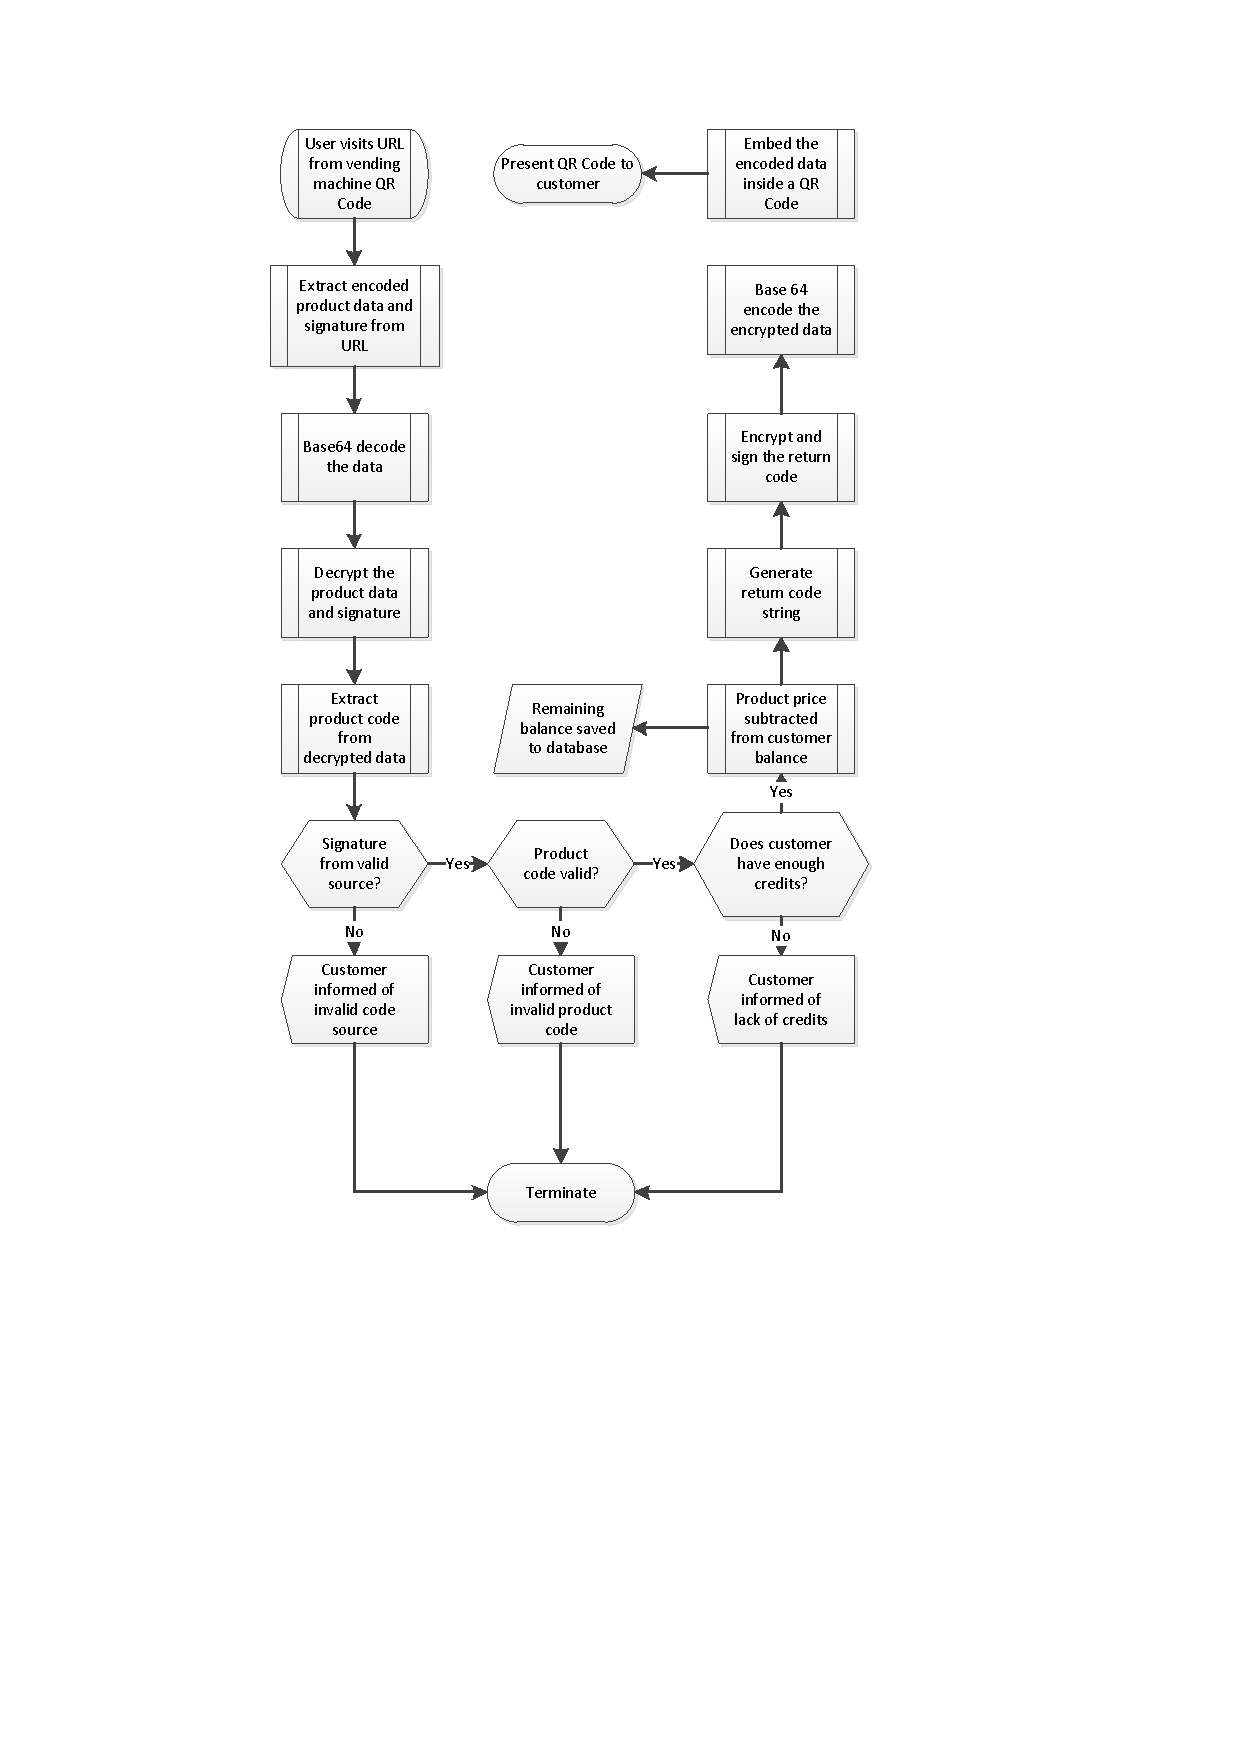
\includegraphics[clip=true, trim = 0 250 0 50,
 scale=0.7]{qrcode_processflow_server_bak}
 \caption{The display\_qrcode app process flow}
 \label{fig:disp-qrcode}
\end{figure}

As seen from Figure \ref{fig:disp-qrcode}, the app first extracts the code containing the
product code and vending machine's signature from the Uniform Resource Locator (URL) that the
customer visited with his cellphone's web browser. The app then proceeds to decode the
the code from the base64 encoded format it was sent in (see Section \ref{sec:base64} on
page \pageref{sec:base64} for some background information on base 64 encoding).

After successfully decoding the data, the app proceeds to decrypt the data and signature with the ElGamal
algorithm using the server's private key and the vending machine's public key
(see Section \ref{sec:assymetric-encryption} on page \pageref{sec:assymetric-encryption} for more detail on
public and private keys) and, following the security code scheme described in Section \ref{sec:security-code-scheme}, extracts the product
code from the decrypted string.

The app then checks to see if the signature comes from a valid source (i.e. one of the vending
machines using this system), if the product code is valid (i.e. the product is in the database)
and if the customer has enough credits loaded loaded onto his account. If either of these
checks return false, an appropriate error message is shown to the customer explaining what
went wrong and what the customer should do next.

If the checks were passed, the app proceeds to subtract the product cost from the user's
remaining balance. Using the security code scheme, the app then generates the correct return
code, encrypts and signs it with the vending machine's public key and the server's private key,
and encodes it with base 64. After this is completed, the app embeds this data into a QR Code,
which is returned to the customer's cellphone screen. 

\subsubsection{load\_money}

This app allows the customer to load money onto his account. At the moment it makes use of
faux money, meaning that the money loaded has no real-world value. The customer can load a
maximum of R1000.00 onto his account.

See Figure \ref{fig:load-money} for the process flow of this
app.

\begin{figure}
 \centering 
 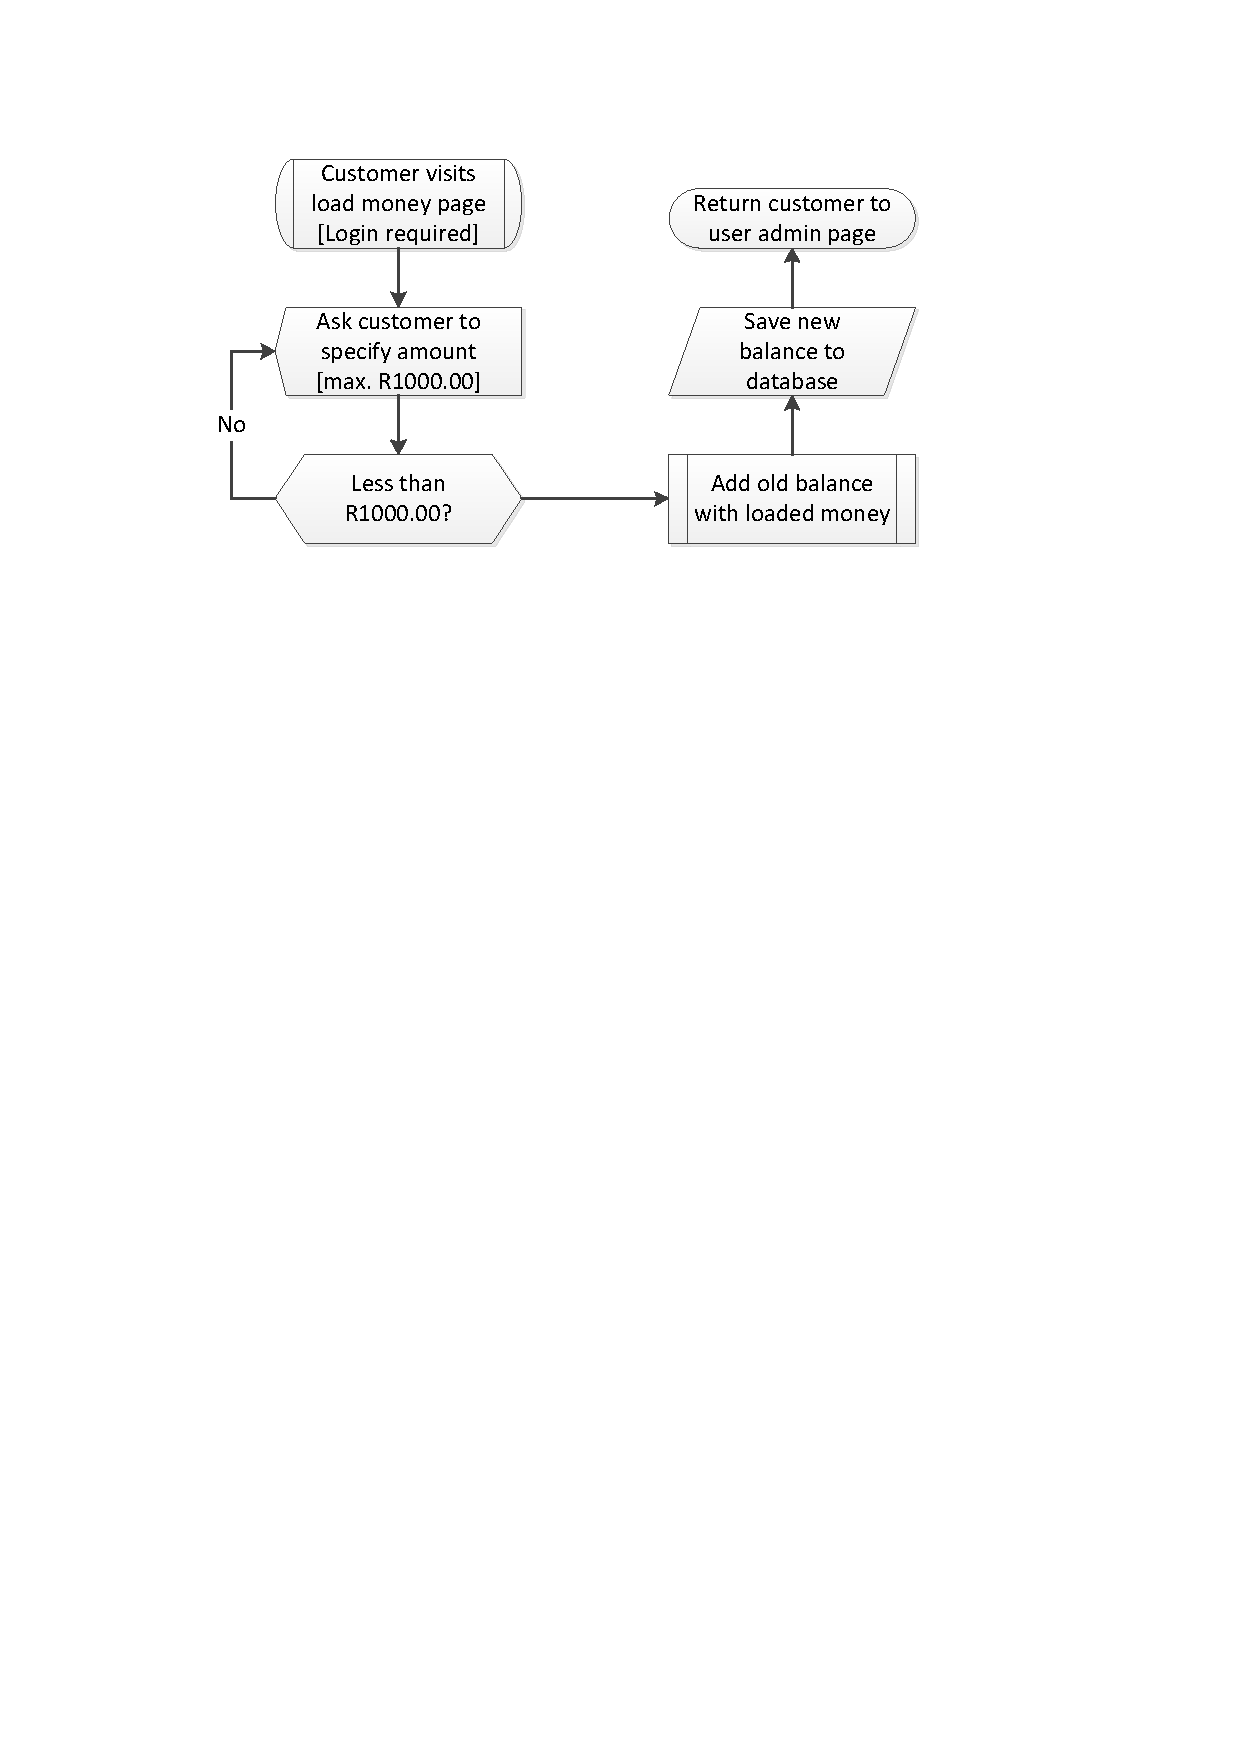
\includegraphics[clip=true, trim = 0 580 100 60,
 scale=0.7]{load_money}
 \caption{The load\_money app process flow}
 \label{fig:load-money}
\end{figure}

\subsubsection{nfc}
\label{sec:app-nfc}

This app forms the core of the NFC payment handling part of the server. See Figure
\ref{fig:nfc-process} for a detailed process flow diagram.

\begin{figure}
 \centering 
 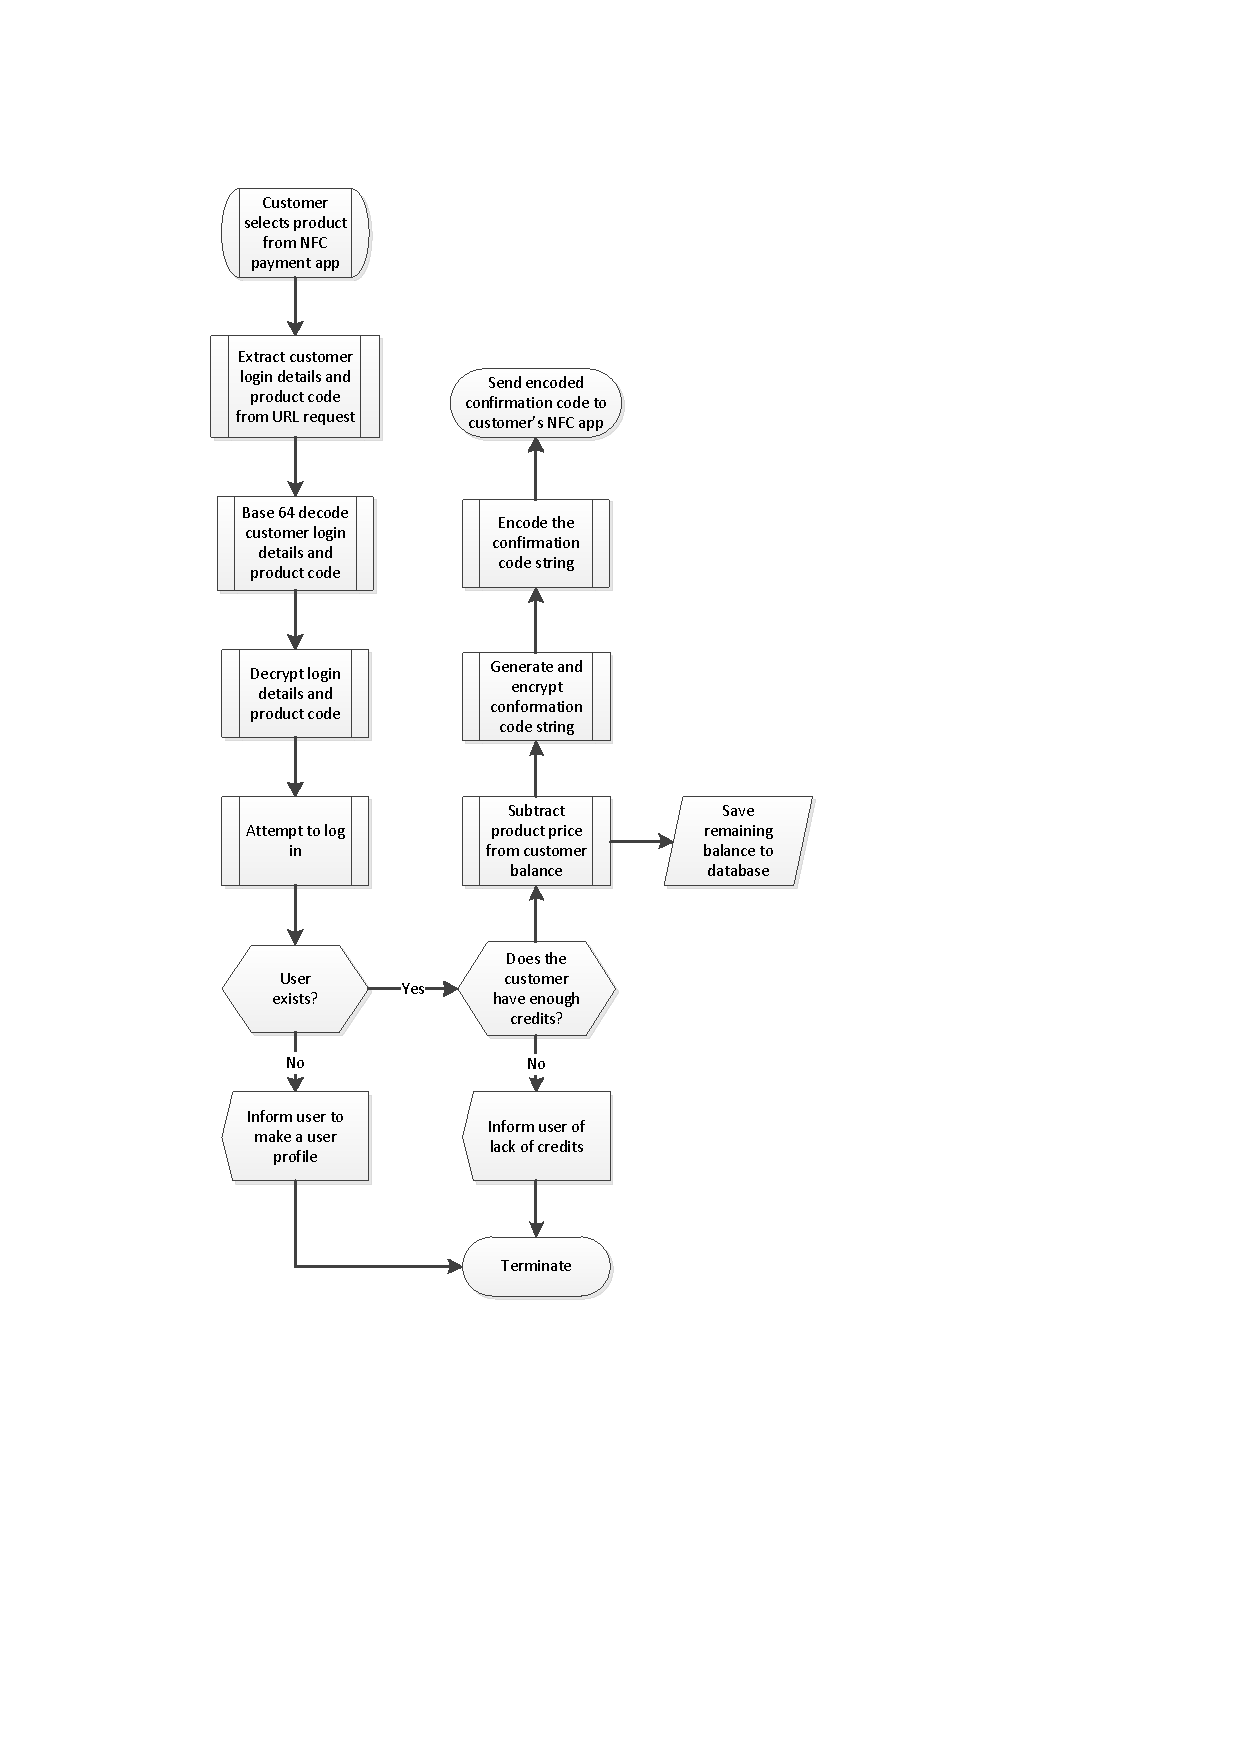
\includegraphics[clip=true, trim = 0 200 100 80,
 scale=0.7]{nfc_processflow_bak}
 \caption{The nfc app process flow}
 \label{fig:nfc-process}
\end{figure}

As seen from Figure \ref{fig:nfc-process}, the server first extracts the encoded and encrypted
customer login details and product code from the URL the NFC app sends to the server. These
codes are then all decoded and decrypted using the Ron Rivest, Adi Shamir and Leonard Adleman
(RSA) algorithm and the server's private key. 

The user login details are then checked and verified using the server's user database. If this
check fails, the customer is given an appropriate error message and informed to create a user
profile. 

If the check is passed, the server then checks to see if the customer has enough money loaded
onto his account. If this check fails, the customer is informed of his lack of funds
and is instructed to load more money. If the check is passed, the server subtracts the product
cost from the customer's balance and encrypts and encodes a confirmation code, according to the
security code scheme specified in Section \ref{sec:security-code-scheme}, which is then sent
to the NFC app. 

\subsubsection{nfc\_add\_user}

This app allows a customer using the NFC app to create a user profile for himself/herself. The
server extracts the customer's login details from the URL request that the NFC app send to the
server. The user name and email are kept in plain text, but the password is decrypted to
plain text with the RSA algorithm and the server's private key.

These details are then saved to the database and is immediately available to be used by the new
customer. 

\subsubsection{register}

This app allows a new customer to register. This app is only accessible by a web browser and
not by the NFC app. However, a user registered with this app will be able to use the same login
details for the NFC app.

The app presents the user with a simple registration page which asks for a user name, email and
password. Using Django's built-in form support. This allows the server to handle the
POST request that is generated when the customer presses the `Continue' button. When this is
done, the login data contained within the POST request is extracted and saved into the user
database. 

\subsection{EC2}

The AWS EC2 server provides the platform on which the Apache
server runs. The EC2 server instance was configured to run
Ubuntu 12.10, `Quantal Quetzal'. This was done because most
of the server development was done on Ubuntu 12.10, and the
server code will therefore require minimal adaptation to be able to run on the EC2 server.

After the server instance was created, the following
packages and programs were installed for the server to be able to run properly:

\begin{itemize}
  \item Apache2: Installs the Apache server framework.
  \item libapache2-mod-wsgi: An Apache module that allows Apache to work with Python wsgi
  scripts.
  \item python-pip: Allows Ubuntu to install Django from the Python Package Index (PyPI)
  [\cite{website:pypi}].
  \item Django: Installs the all the Django packages that will be used by the server. 
\end{itemize}

Because the server's database uses SQLite3, and Ubuntu 12.10 comes with it by default, no
external database programs were needed to be installed. 

After this was completed, the server is fully capable of serving Django web
pages.

\subsection{Apache}

The Apache server framework provides the foundation on which the Django server runs. It had to
be configured to be able to run the Python scripts that Django contains. To do this, the steps
described in Nick Polet's blog post was followed [\cite{article:apache-setup}]. It describes
in detail how to configure Apache to serve a Django website.

For Apache to be able to serve Django sites, it had to be configured to run the Web Server
Gateway Interface (wsgi.py) script located within the Django server folder. This was done by
adding the following code to the Apache's httpd.conf configuration file:

\begin{verbatim}
WSGIScriptAlias / /home/ubuntu/srv/server_site/server_site/wsgi.py
WSGIPythonPath /home/ubuntu/srv/server_site

<Directory /home/ubuntu/srv/server_site/server_site>
<Files wsgi.py>
Order deny,allow
Allow from all
</Files>
</Directory>
\end{verbatim}

The following line was also needed to be added to Apache's apache2.conf file:

\begin{verbatim}
Include httpd.conf
\end{verbatim}

\section{Vending Program}

The vending machine's program runs the vending machine. It is responsible for
allowing the customer to select a product, to create a QR Code for that takes the customer
to the web server, to scan the customer's response QR Code, to scan the customer's NFC
request and to dispense the product after a successful transaction. 

The whole program is based on Python scripts and
designed to be used by a Raspberry Pi microcomputer (see Section
\ref{sec:raspi} on page \pageref{sec:raspi} for more details on the Raspberry Pi). The whole
transaction process is given in Figure \ref{fig:vm_prog_interaction}.

\begin{figure}
 \centering 
 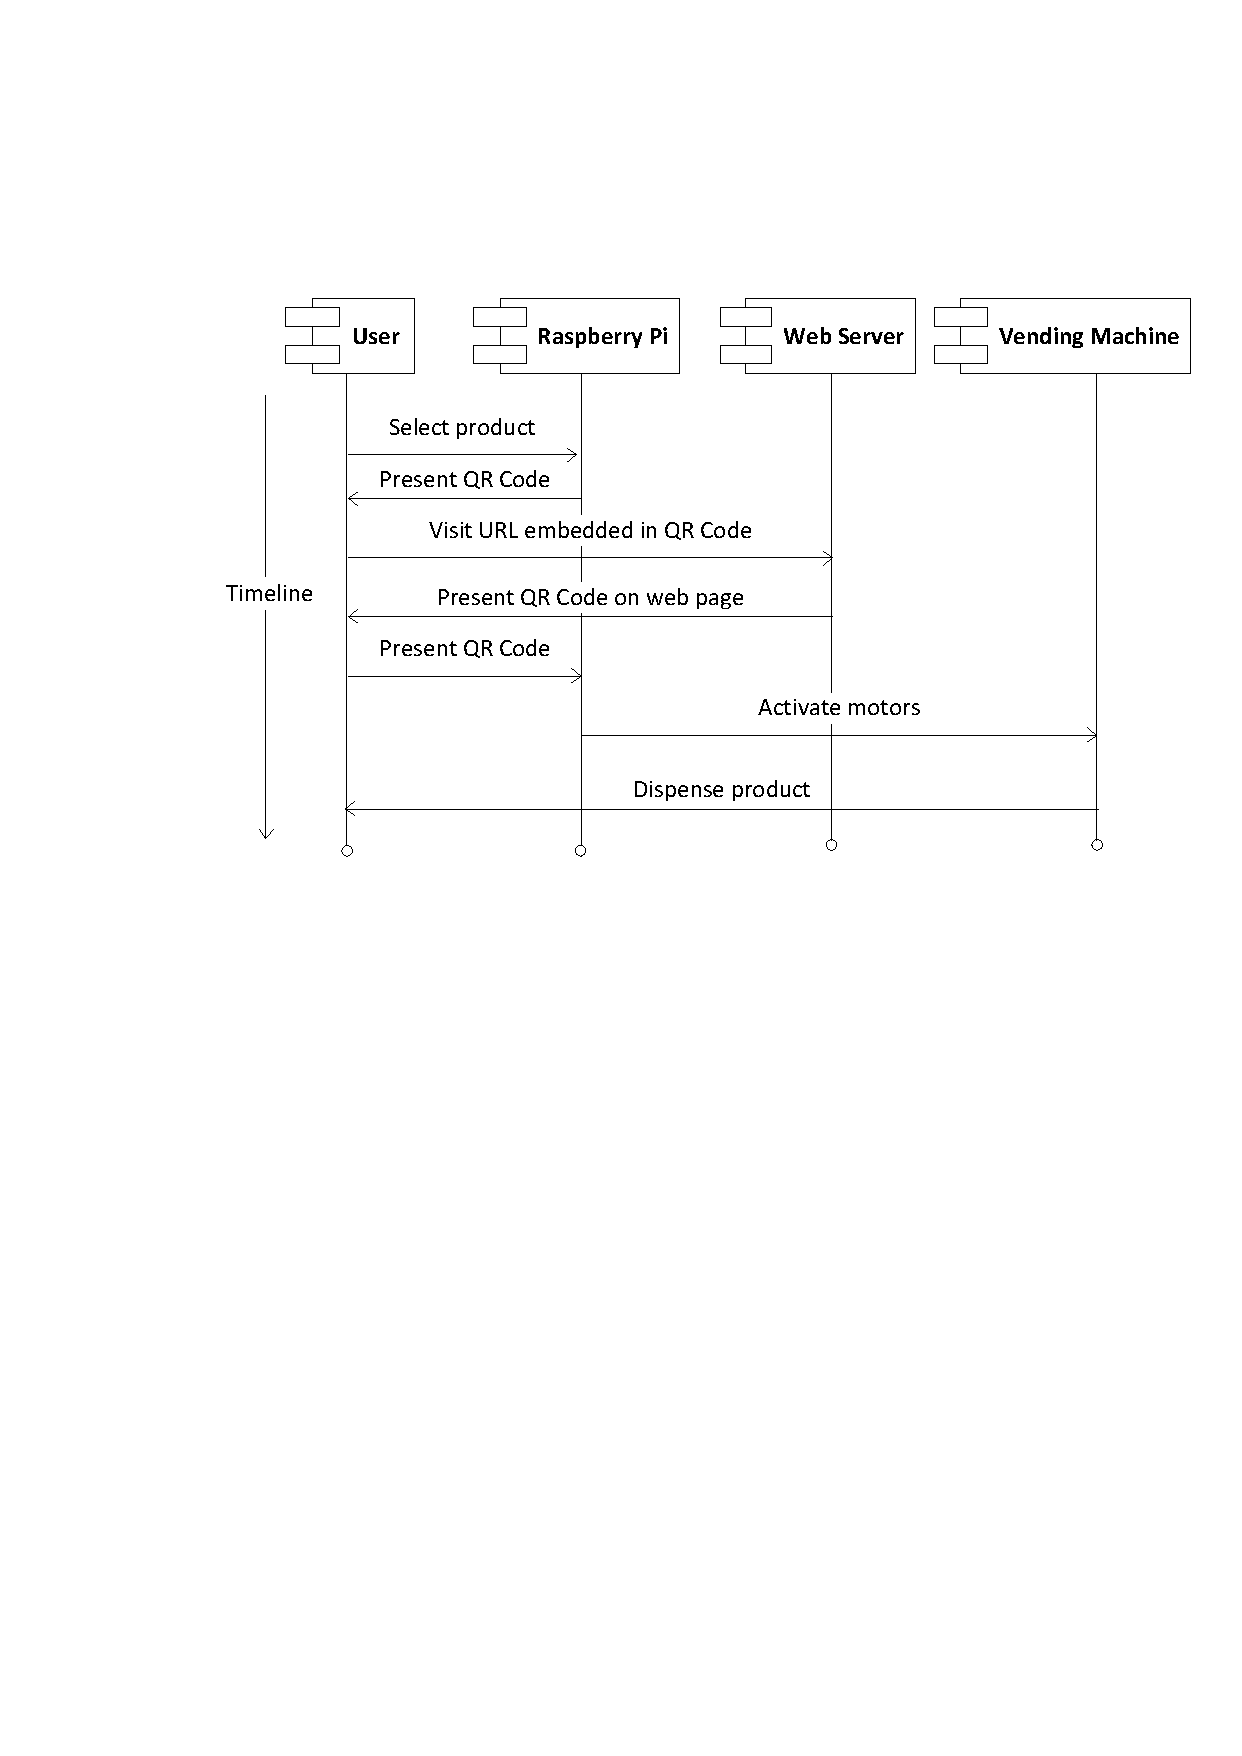
\includegraphics[clip=true, trim = 50 400 0 140, scale=0.7]{qrcode_processflow_user}
 \caption{The vending machine transaction process}
 \label{fig:vm_prog_interaction}
\end{figure}

To simplify the program, its split up into separate sub-programs. These
sub-programs, called scripts, are discussed in this section.

The program structure can be seen in Figure
\ref{fig:vm_prog_strcture}.

\begin{figure}
 \centering 
 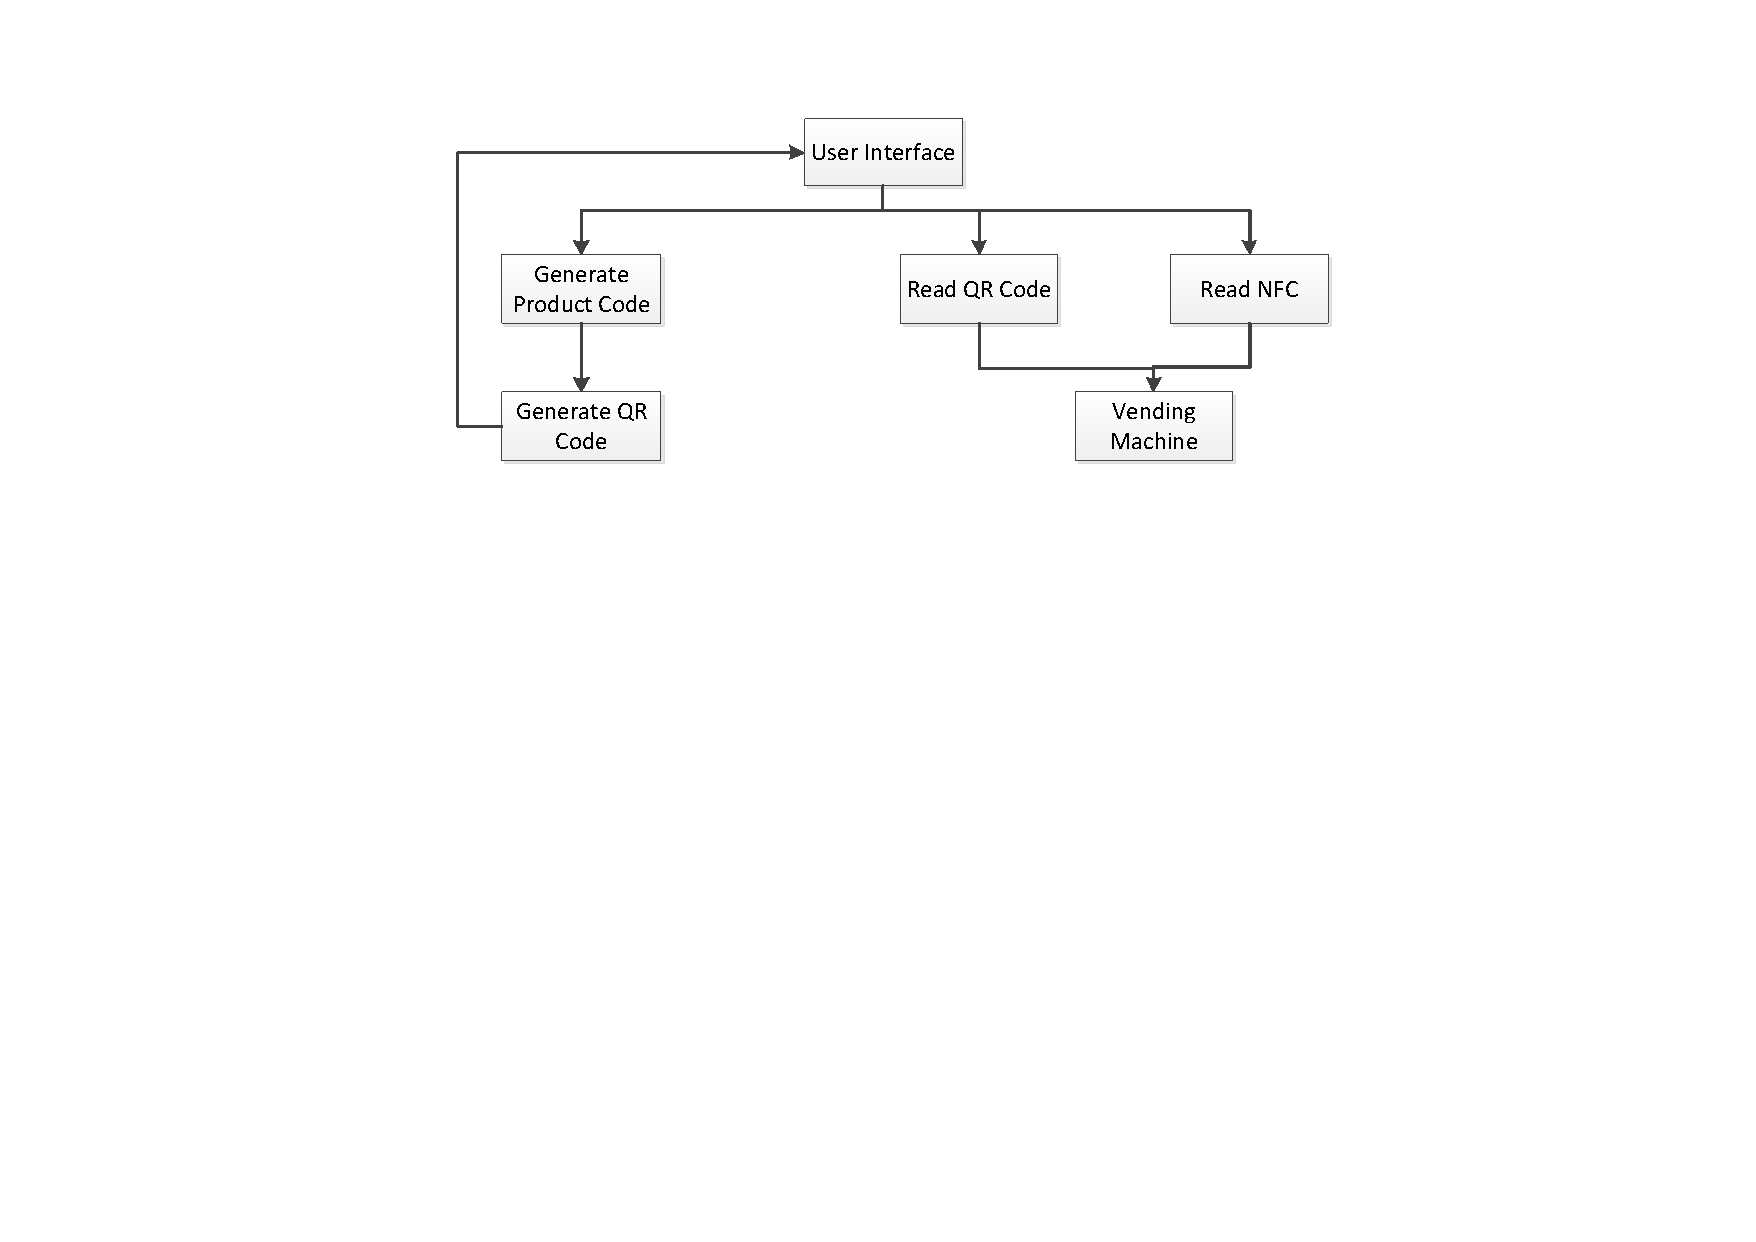
\includegraphics[clip=true, trim = 100 320 0 50,
 scale=0.7]{vending_machine_program_structure}
 \caption{The vending machine's program structure}
 \label{fig:vm_prog_strcture}
\end{figure}

\subsection{User Interface}

To allow the customer to select a product, a Graphical User Interface (GUI) was
created. The GUI was made using the WX Python GUI toolkit
[\cite{website:wx-python}].
See Figure \ref{fig:gui-screenshot} for a screenshot of the
GUI.

\begin{figure}
 \centering 
 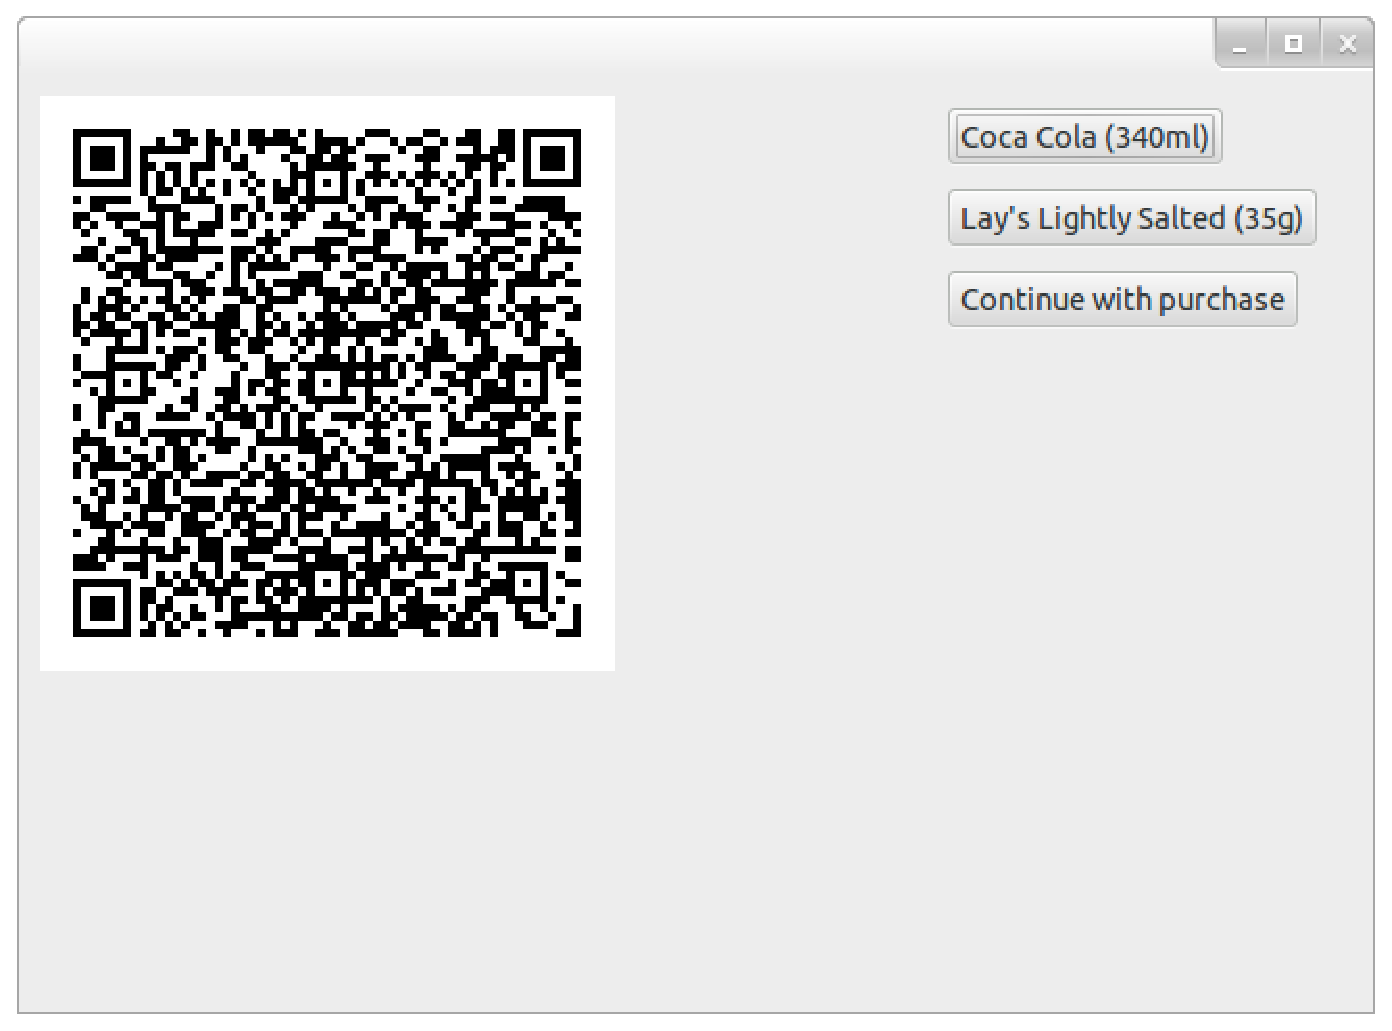
\includegraphics[scale=0.4]{gui_screenshot}
 \caption{A screenshot of the user interface}
 \label{fig:gui-screenshot}
\end{figure}

As can be seen from Figure \ref{fig:vm_prog_strcture}, the GUI script is
responsible for calling the encryption script and the QR Code generation script.
It is also responsible for displaying the QR Code, to handle transactions from
the Android NFC app and to activate the correct motor inside the vending
machine. 

\subsection{Generating a Product Code}

After the customer selects which product to buy from the GUI, the
encrypt\_elgamal script is called. This script is responsible for generating the
random hex character string, in accordance with the security scheme described in
Section \ref{sec:security-code-scheme}, encrypting, signing and encoding the
string in base 64 and embedding the random string inside a Uniform
Resource Locator (URL) that points to the web server. This URL is then sent to
the generate\_qrcode script described in Section \ref{sec:gen-qrcode}.

See Figure \ref{fig:gen-prod-code-processflow} for a detailed process flow
diagram.

\begin{figure}
 \centering 
 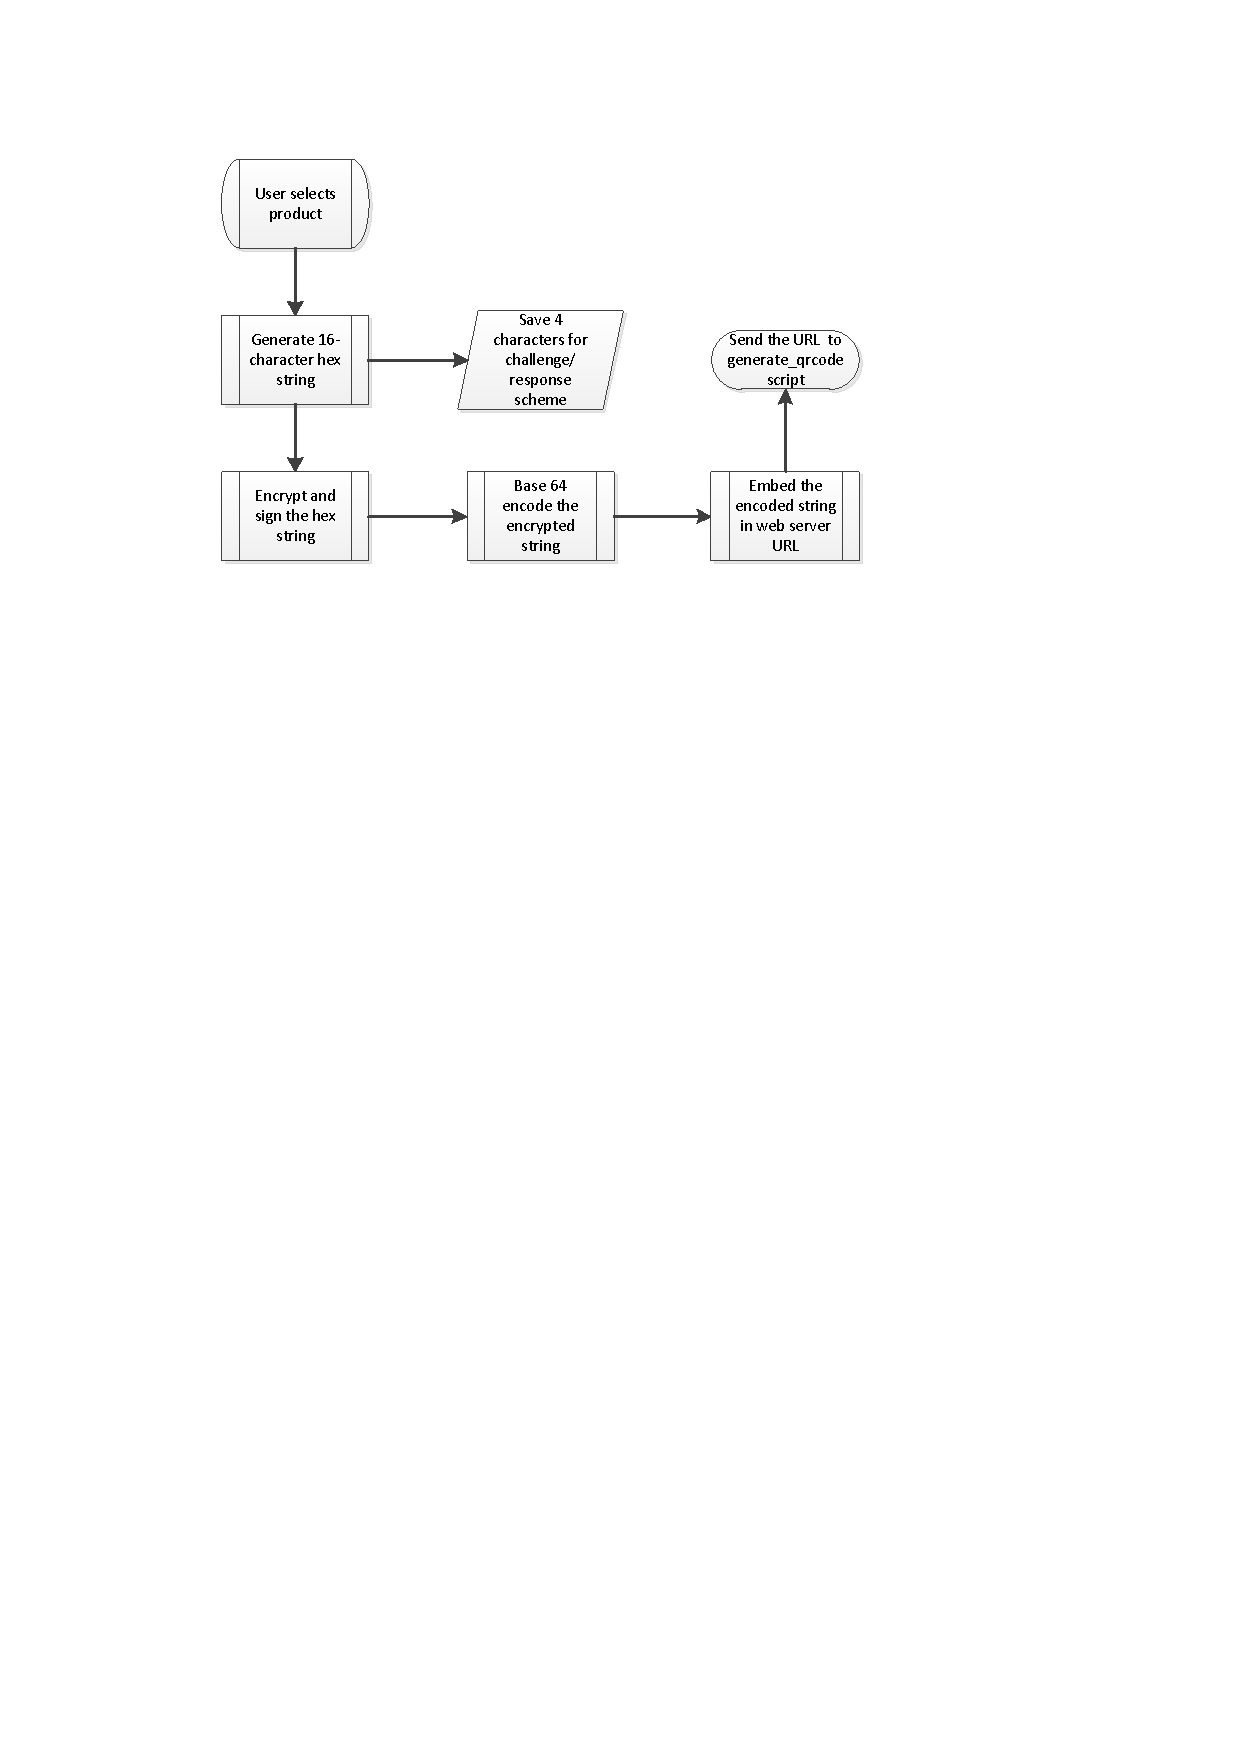
\includegraphics[clip=true, trim
 = 0 550 0 70, scale=0.7]{generate_product_code_processflow}
 \caption{The GUI process flow}
 \label{fig:gen-prod-code-processflow}
\end{figure}

\subsection{Generating a QR Code}
\label{sec:gen-qrcode}

After the encrypt\_elgamal script has been run, the generate\_qrcode script is
called. This script is responsible for embedding the URL received from the
encrypt\_elgamal script into a QR Code. This is done by using a qrcode module
for Python, called qrcode [\cite{website:qrcode-generator}].

\subsection{Reading a QR Code}

After the customer has received his QR Code from the server verifying the
transaction, the customer may press the button called `Continue with purchase'.
When this is done the read\_qrcode script is run.

This script is responsible for reading the customer's QR Code via a web cam,
extract the data from the scanned image, decrypting the data and verifying the
transaction. See Figure \ref{fig:read-qrcode-processflow} for a detailed process
flow diagram.

\begin{figure}
 \centering 
 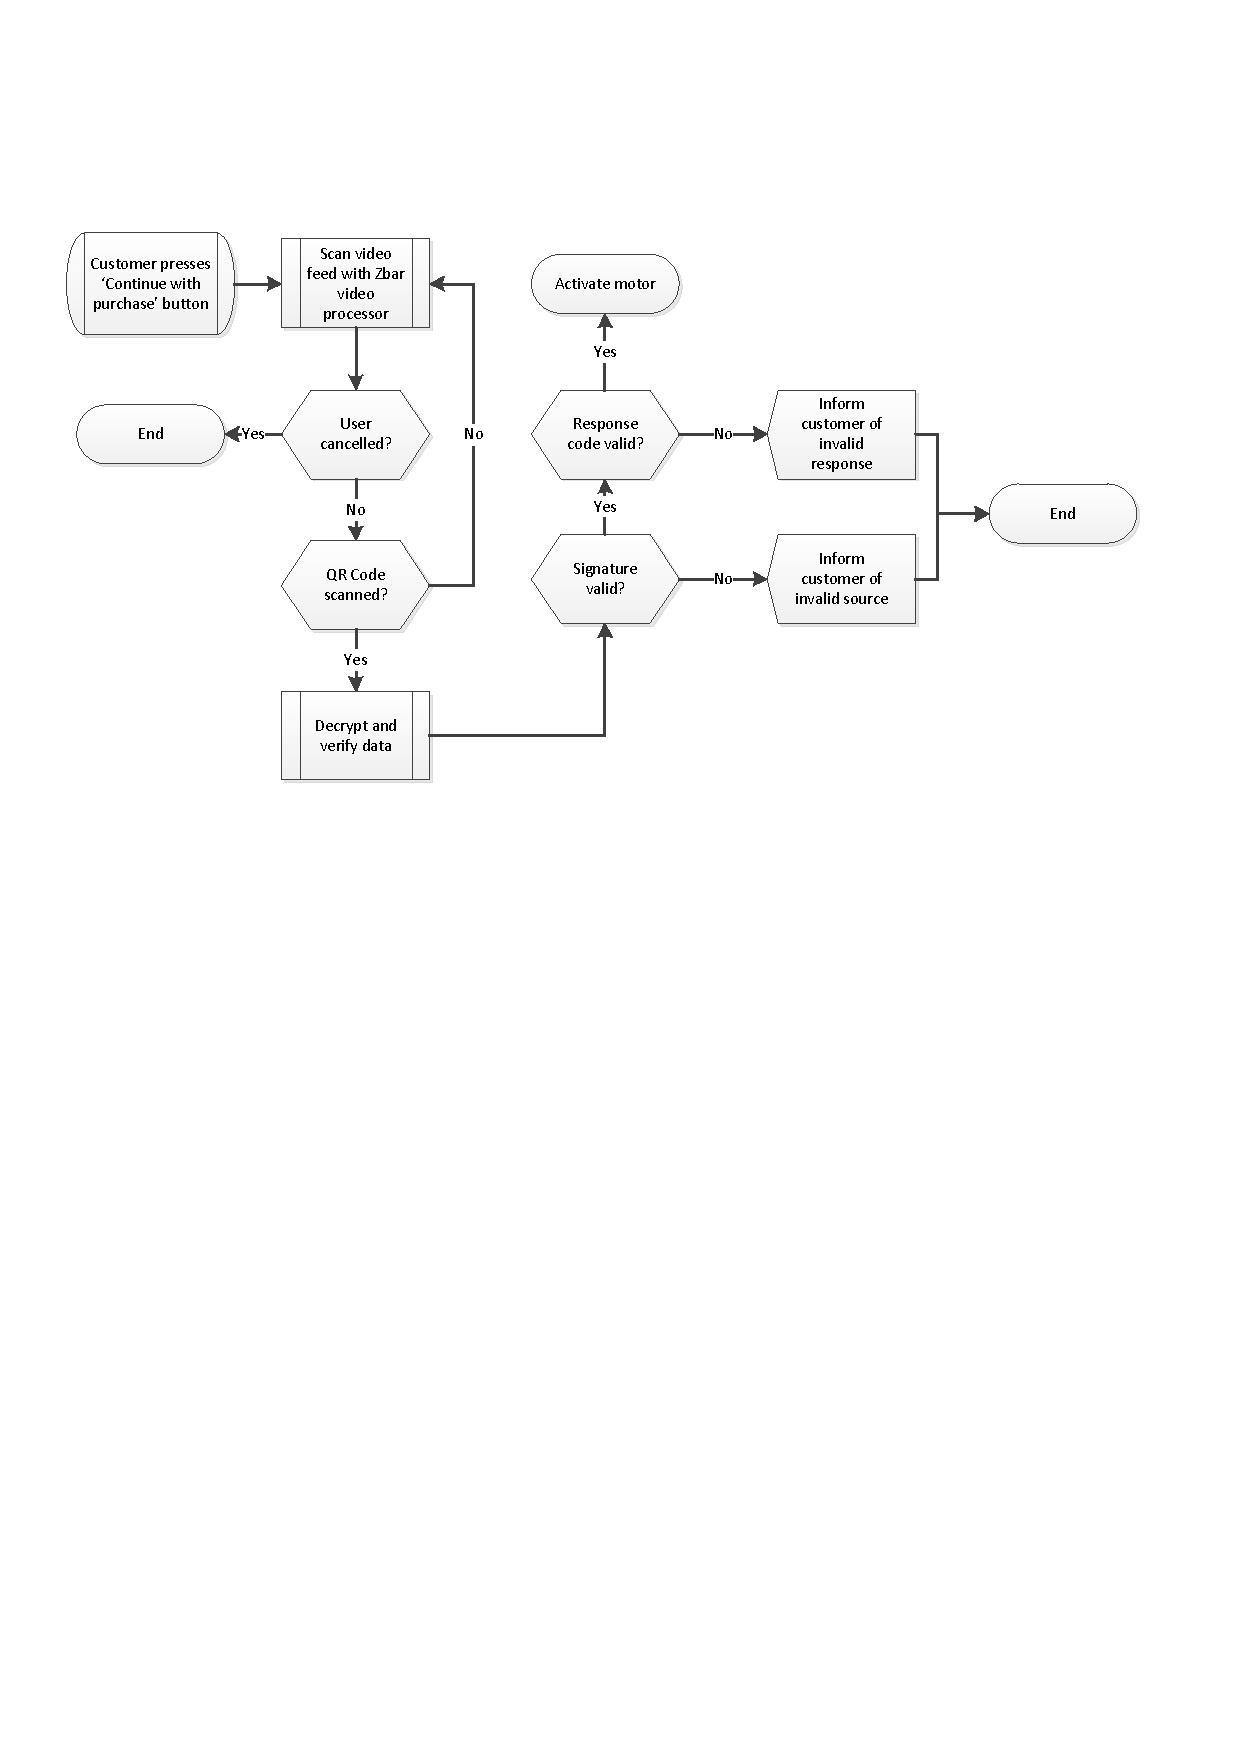
\includegraphics[clip=true, trim
 = 0 460 0 100, scale=0.75]{read_qrcode_processflow}
 \caption{The generate\_qrcode script process flow}
 \label{fig:read-qrcode-processflow}
\end{figure}

As seen from Figure \ref{fig:read-qrcode-processflow}, as soon as the `Continue
with purchase' button is pressed, the script creates a ZBar image processor
which scans a web cam video feed for a QR Code (see Section \ref{sec:zbar} on page
\pageref{sec:zbar} for more information on ZBar). This image processor runs until the user
cancels the process or it scans a QR Code. 

After the ZBar processor has scanned a QR Code, it sends the retrieved data to
be decrypted and verified with the ElGamal algorithm and the vending machine's
private key and the server's public key. If the signature is valid and the data
contains a valid response and product code, the script activates the correct
motor and the customer receives his product. 

\subsection{Near Field Communication}

If the customer opts to purchase a product with the Android Near Field
Communication (NFC) app, the NFC script is run. This script is based on an
example script included in the nfcpy package (see Section \ref{sec:nfcpy} on page
\pageref{sec:nfcpy} for more detail) and is written by nfcpy's creator, Stephen Tiedemann
[\cite{website:nfcpy}]. This example script, called snep-test-server, does the
following:

\begin{itemize}
  \item It connects the Raspberry Pi to the NFC controller chip.
  \item It polls the NFC controller chip for a Simple NFC Data Exchange Format
  Exchange Protocol (SNEP) message.
  \item When a SNEP message is read, it extracts the data in the message and
  presents it to the programmer for further processing and manipulation.
\end{itemize}

Using this example script allows the vending machine to extract SNEP messages
from any source that follows the NFC Forum's standards
[\cite{website:nfc-forum}]. For this project, an Android NFC app was written
specifically for this purpose (see Section \ref{sec:nfc-android-app} for more
detail). 

After the data is extracted from the NFC source, the script decrypts the data
using the RSA algorithm and the vending machine's private key. The vending
machine then checks the NFC message's response code. 

If the response code is valid, the script then activates the correct motor to
dispense the product to the customer.

\section{Android Application}
\label{sec:nfc-android-app}

An Android NFC app was made for this project. It allows a customer to buy a
product from the app's product menu and to complete the purchase by swiping
his phone across the vending machine's NFC receiver.

The app is divided up into three activities (Android's technical term for what
is essentially a different window of the app). 

These activities, their design and significance are discussed in this section.

See Figure \ref{fig:nfc_app_structure} for a structure
diagram of the app.

\begin{figure}
 \centering 
 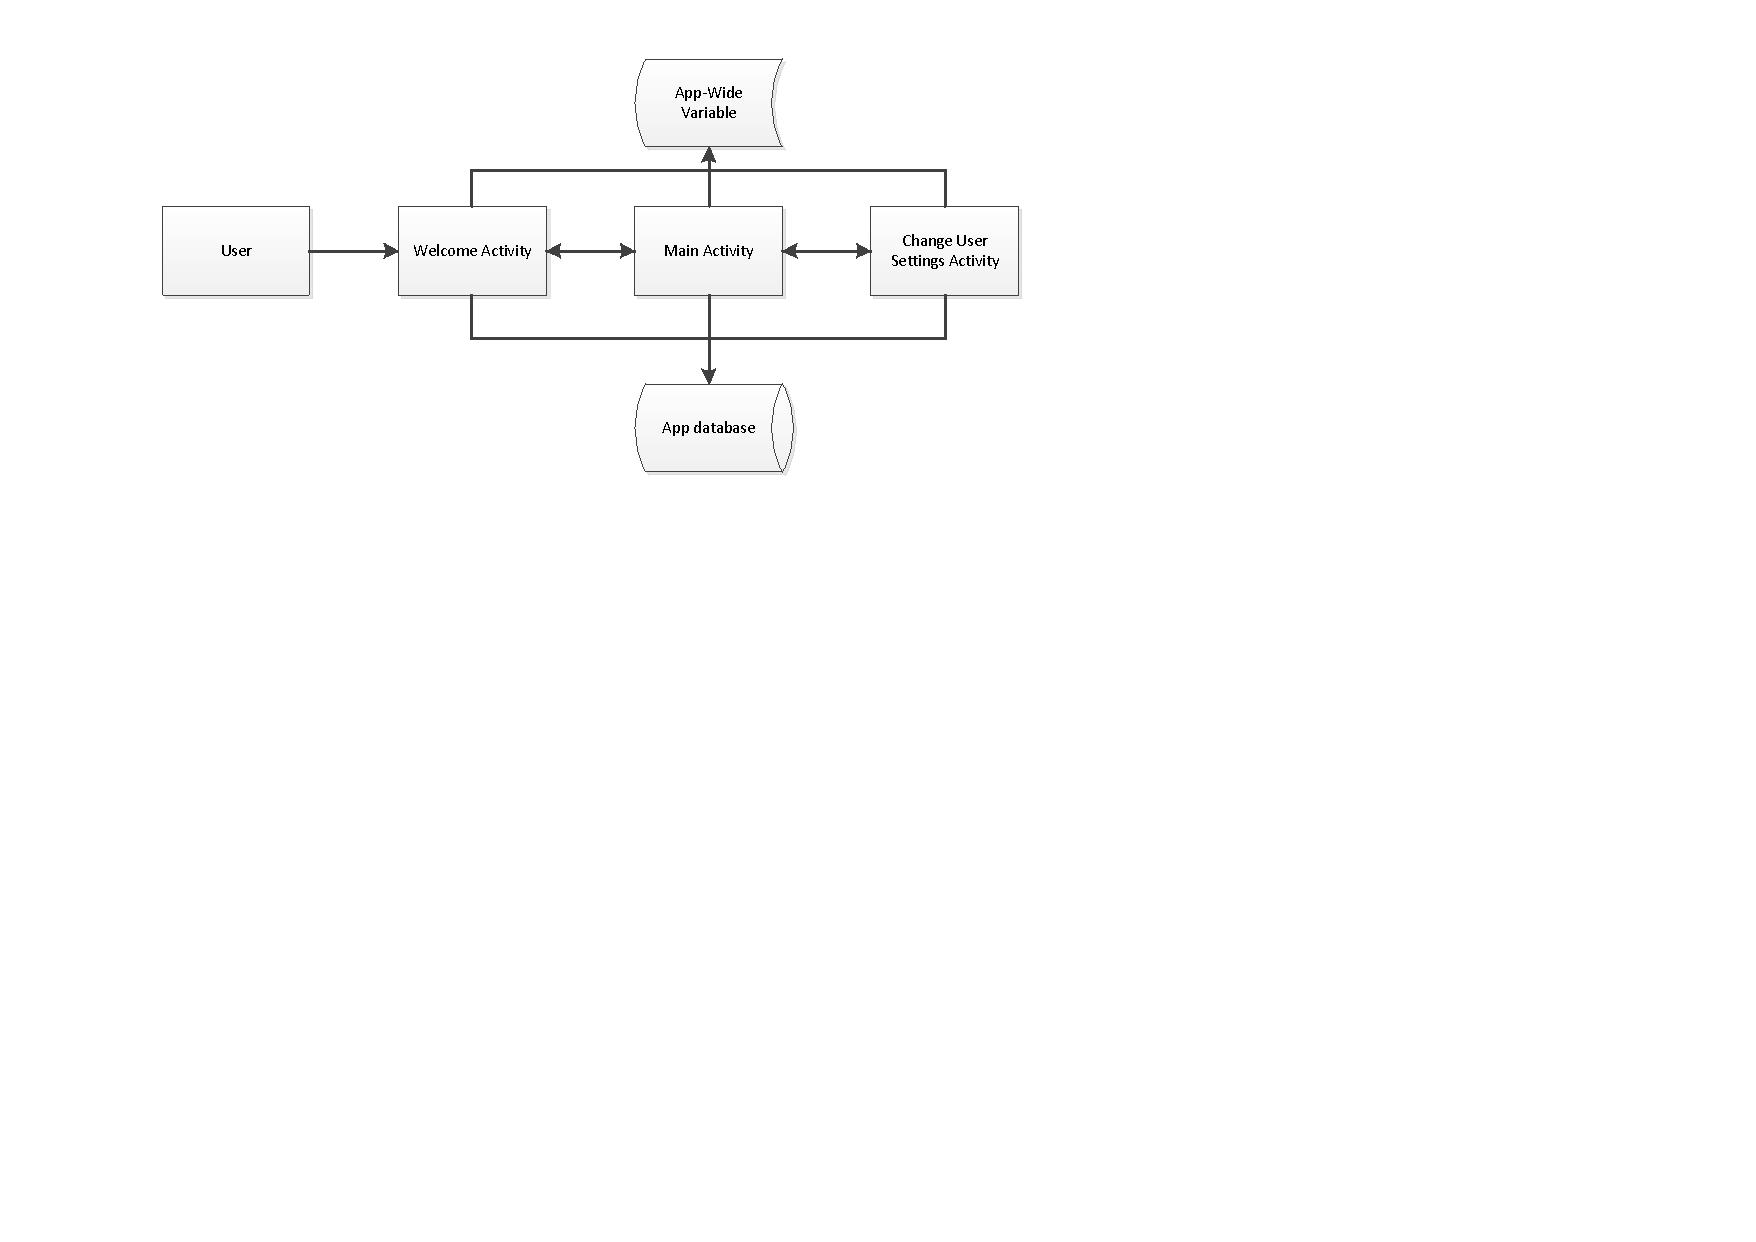
\includegraphics[clip = true, trim = 0 360 0 20,
 scale=0.7]{app_structure}
 \caption{The Android NFC app structure}
 \label{fig:nfc_app_structure}
\end{figure}

\subsection{Welcome Screen}

This activity is the activity that is called when the app is opened. This
activities process flow can be seen in Figure \ref{fig:app-welcomescreen}.
Figure \ref{fig:welcomescreen-screenshot} shows a screenshot of the welcome
screen.

\begin{figure}
 \centering 
 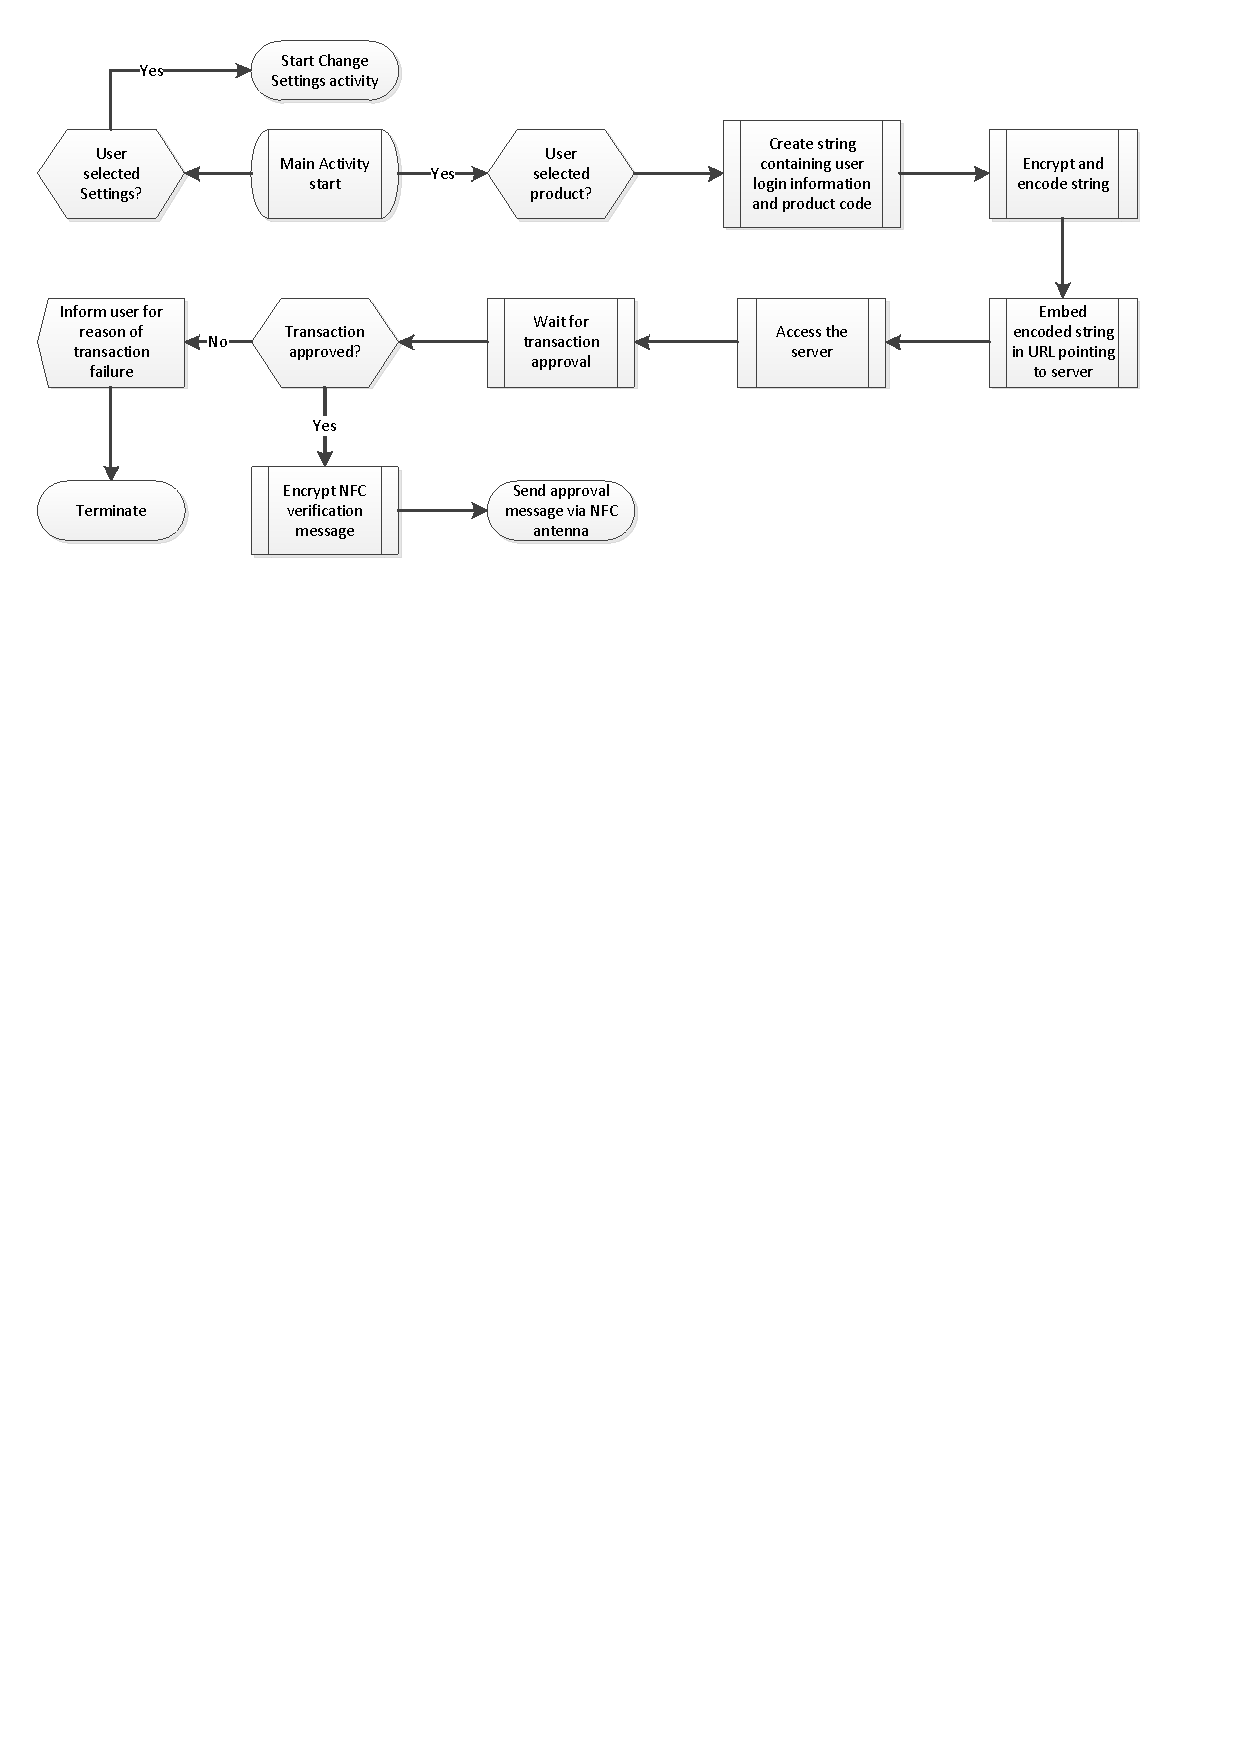
\includegraphics[clip = true, trim = 0 550 0 0,
 scale=0.75]{app_main_processflow}
 \caption{The Android NFC app structure}
 \label{fig:app-welcomescreen}
\end{figure}

\begin{figure}[h]
 \centering 
 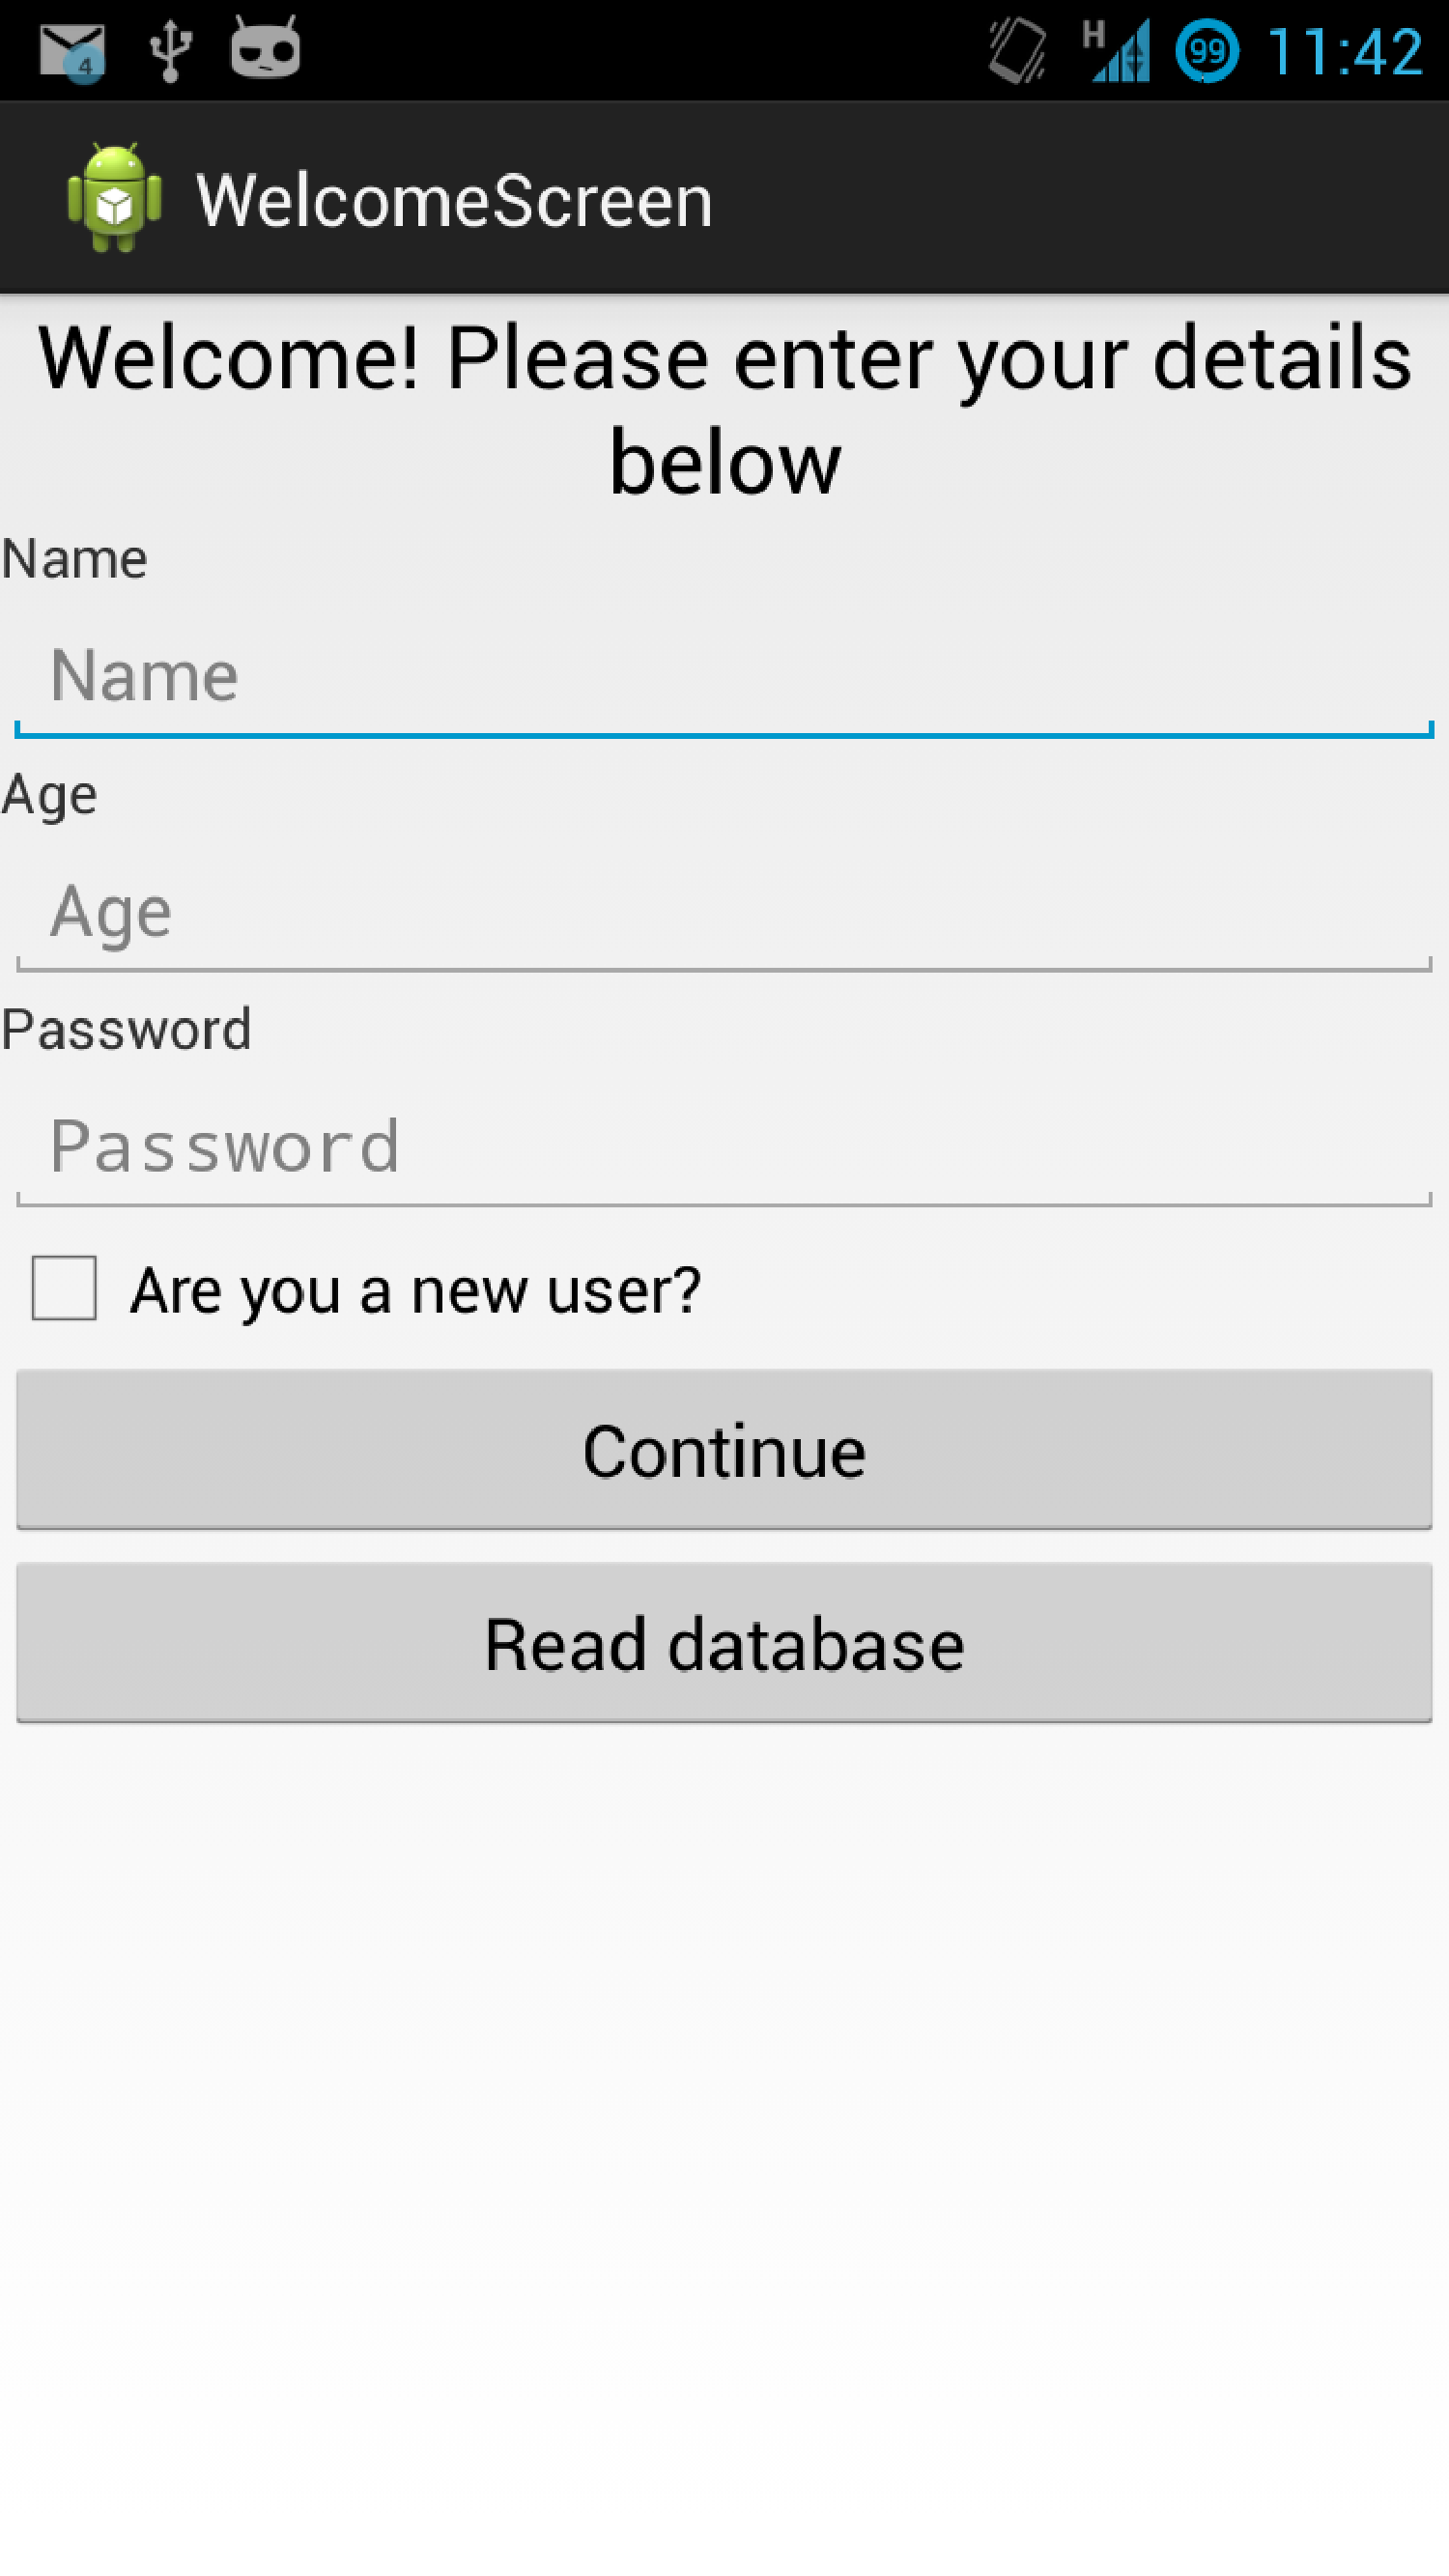
\includegraphics[clip = true, trim = 0 320 0 60, scale=0.2]{welcome_screen}
 \caption{A screenshot of the app's welcome screen}
 \label{fig:welcomescreen-screenshot}
\end{figure}

As seen from Figure \ref{fig:app-welcomescreen}, the
activity first checks to see if its the first time the user opens the app. If its not,
the activity goes on to the Main Activity. Otherwise, it allows the user to either sign
in with an existing profile or create a new one.

When the user signs into an existing profile, the login details he/she provides
is stored in a database that is only accessible by this app. When this is done, it
makes the login information persistent throughout the lifetime of the app.

These details are also saved into an app-wide variable. This variable is
only accessible by the app and is only active while the app is running in
the foreground or background. This variable is used to make the app more
efficient by not having to read the database every time the user wants to use
the app. This variable is only active while the app is running in the foreground
or background

The login details saved here are used later by the app's other activities.

\subsection{Change User Settings}

The Change User Settings activity allows the user to change his login
details that are saved in the database and the app-wide variable. See Figure
\ref{fig:change-user-settings} for a detailed process flow diagram for this
activity. Figure \ref{fig:change-settings-screenshot} shows a screenshot of this
activity.

\begin{figure}
 \centering 
 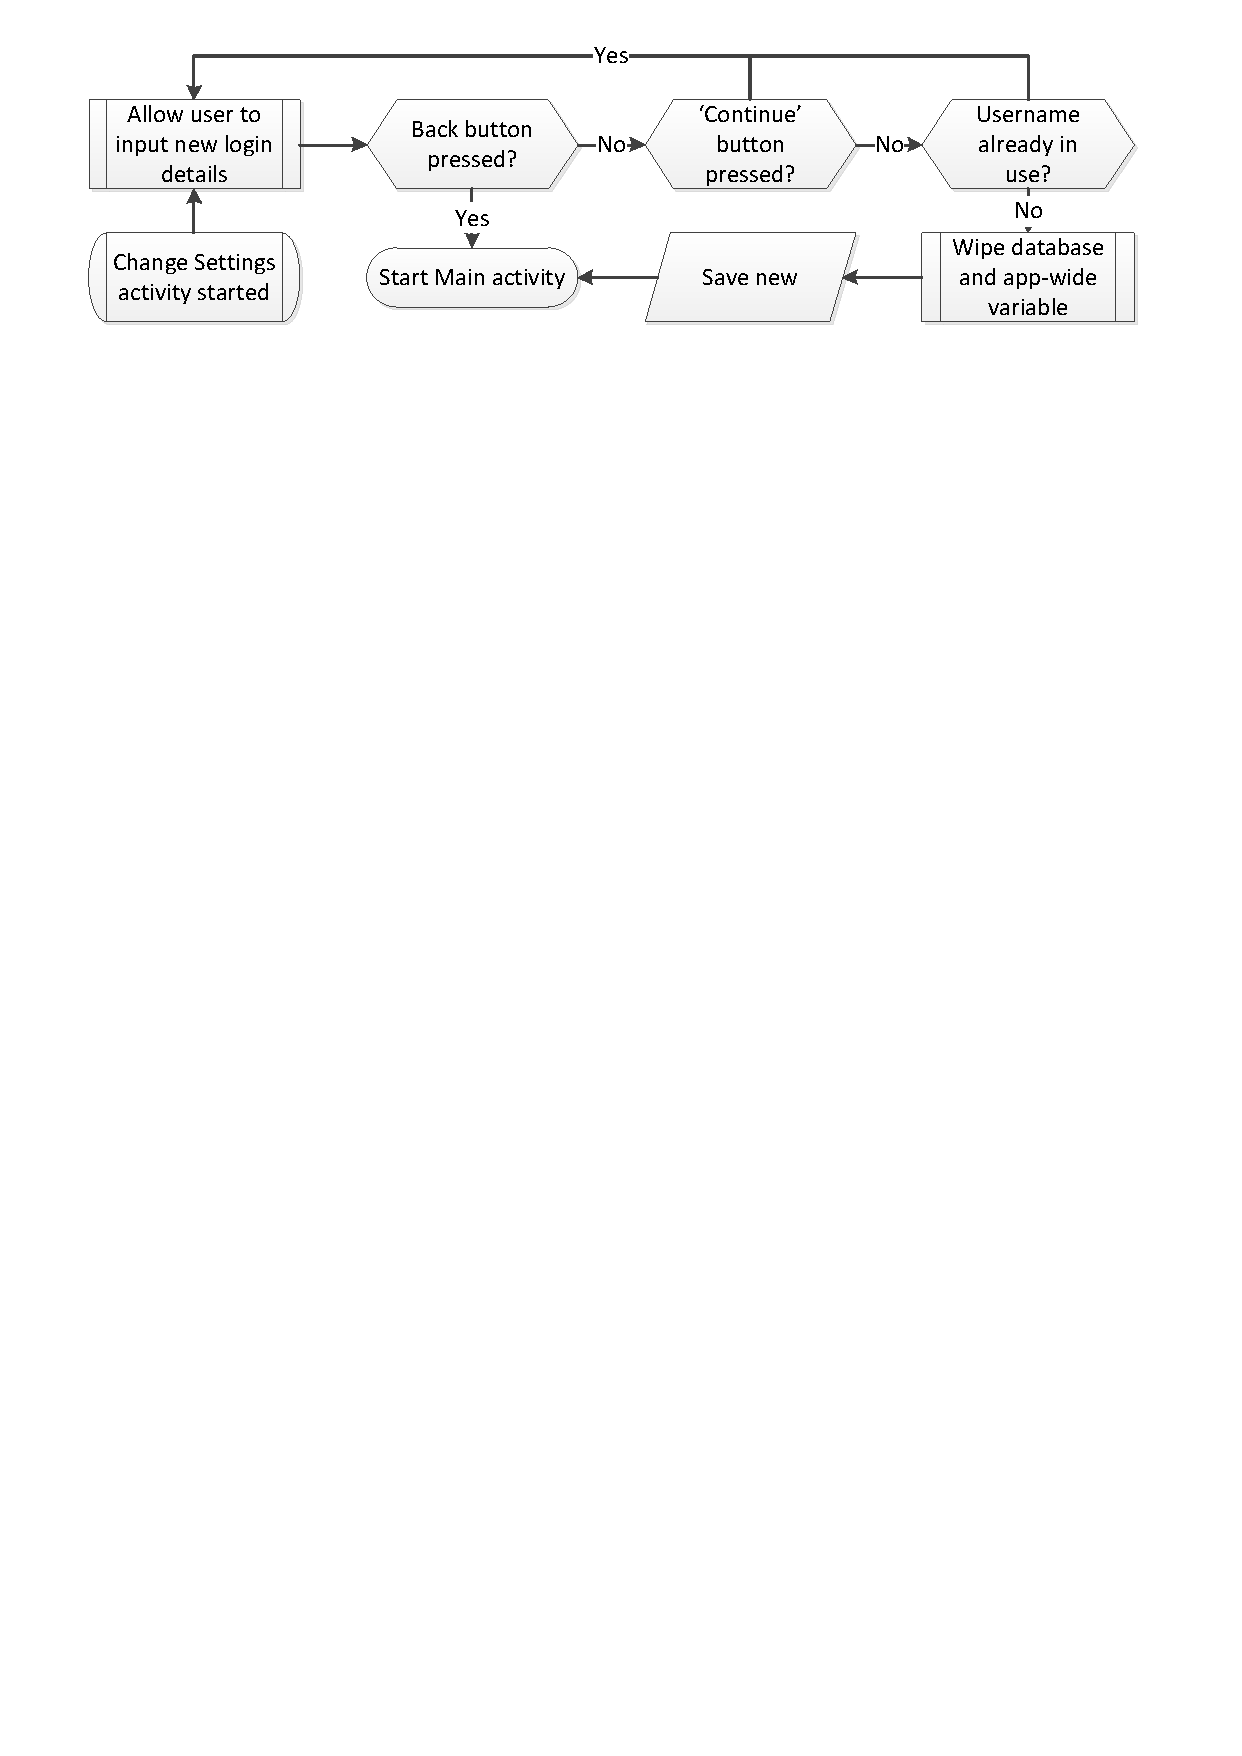
\includegraphics[clip = true, trim = 0 650 0 0,
 scale=0.7]{change_settings_processflow}
 \caption{The process flow of the Change Settings activity}
 \label{fig:change-user-settings}
\end{figure}

\begin{figure}
 \centering 
 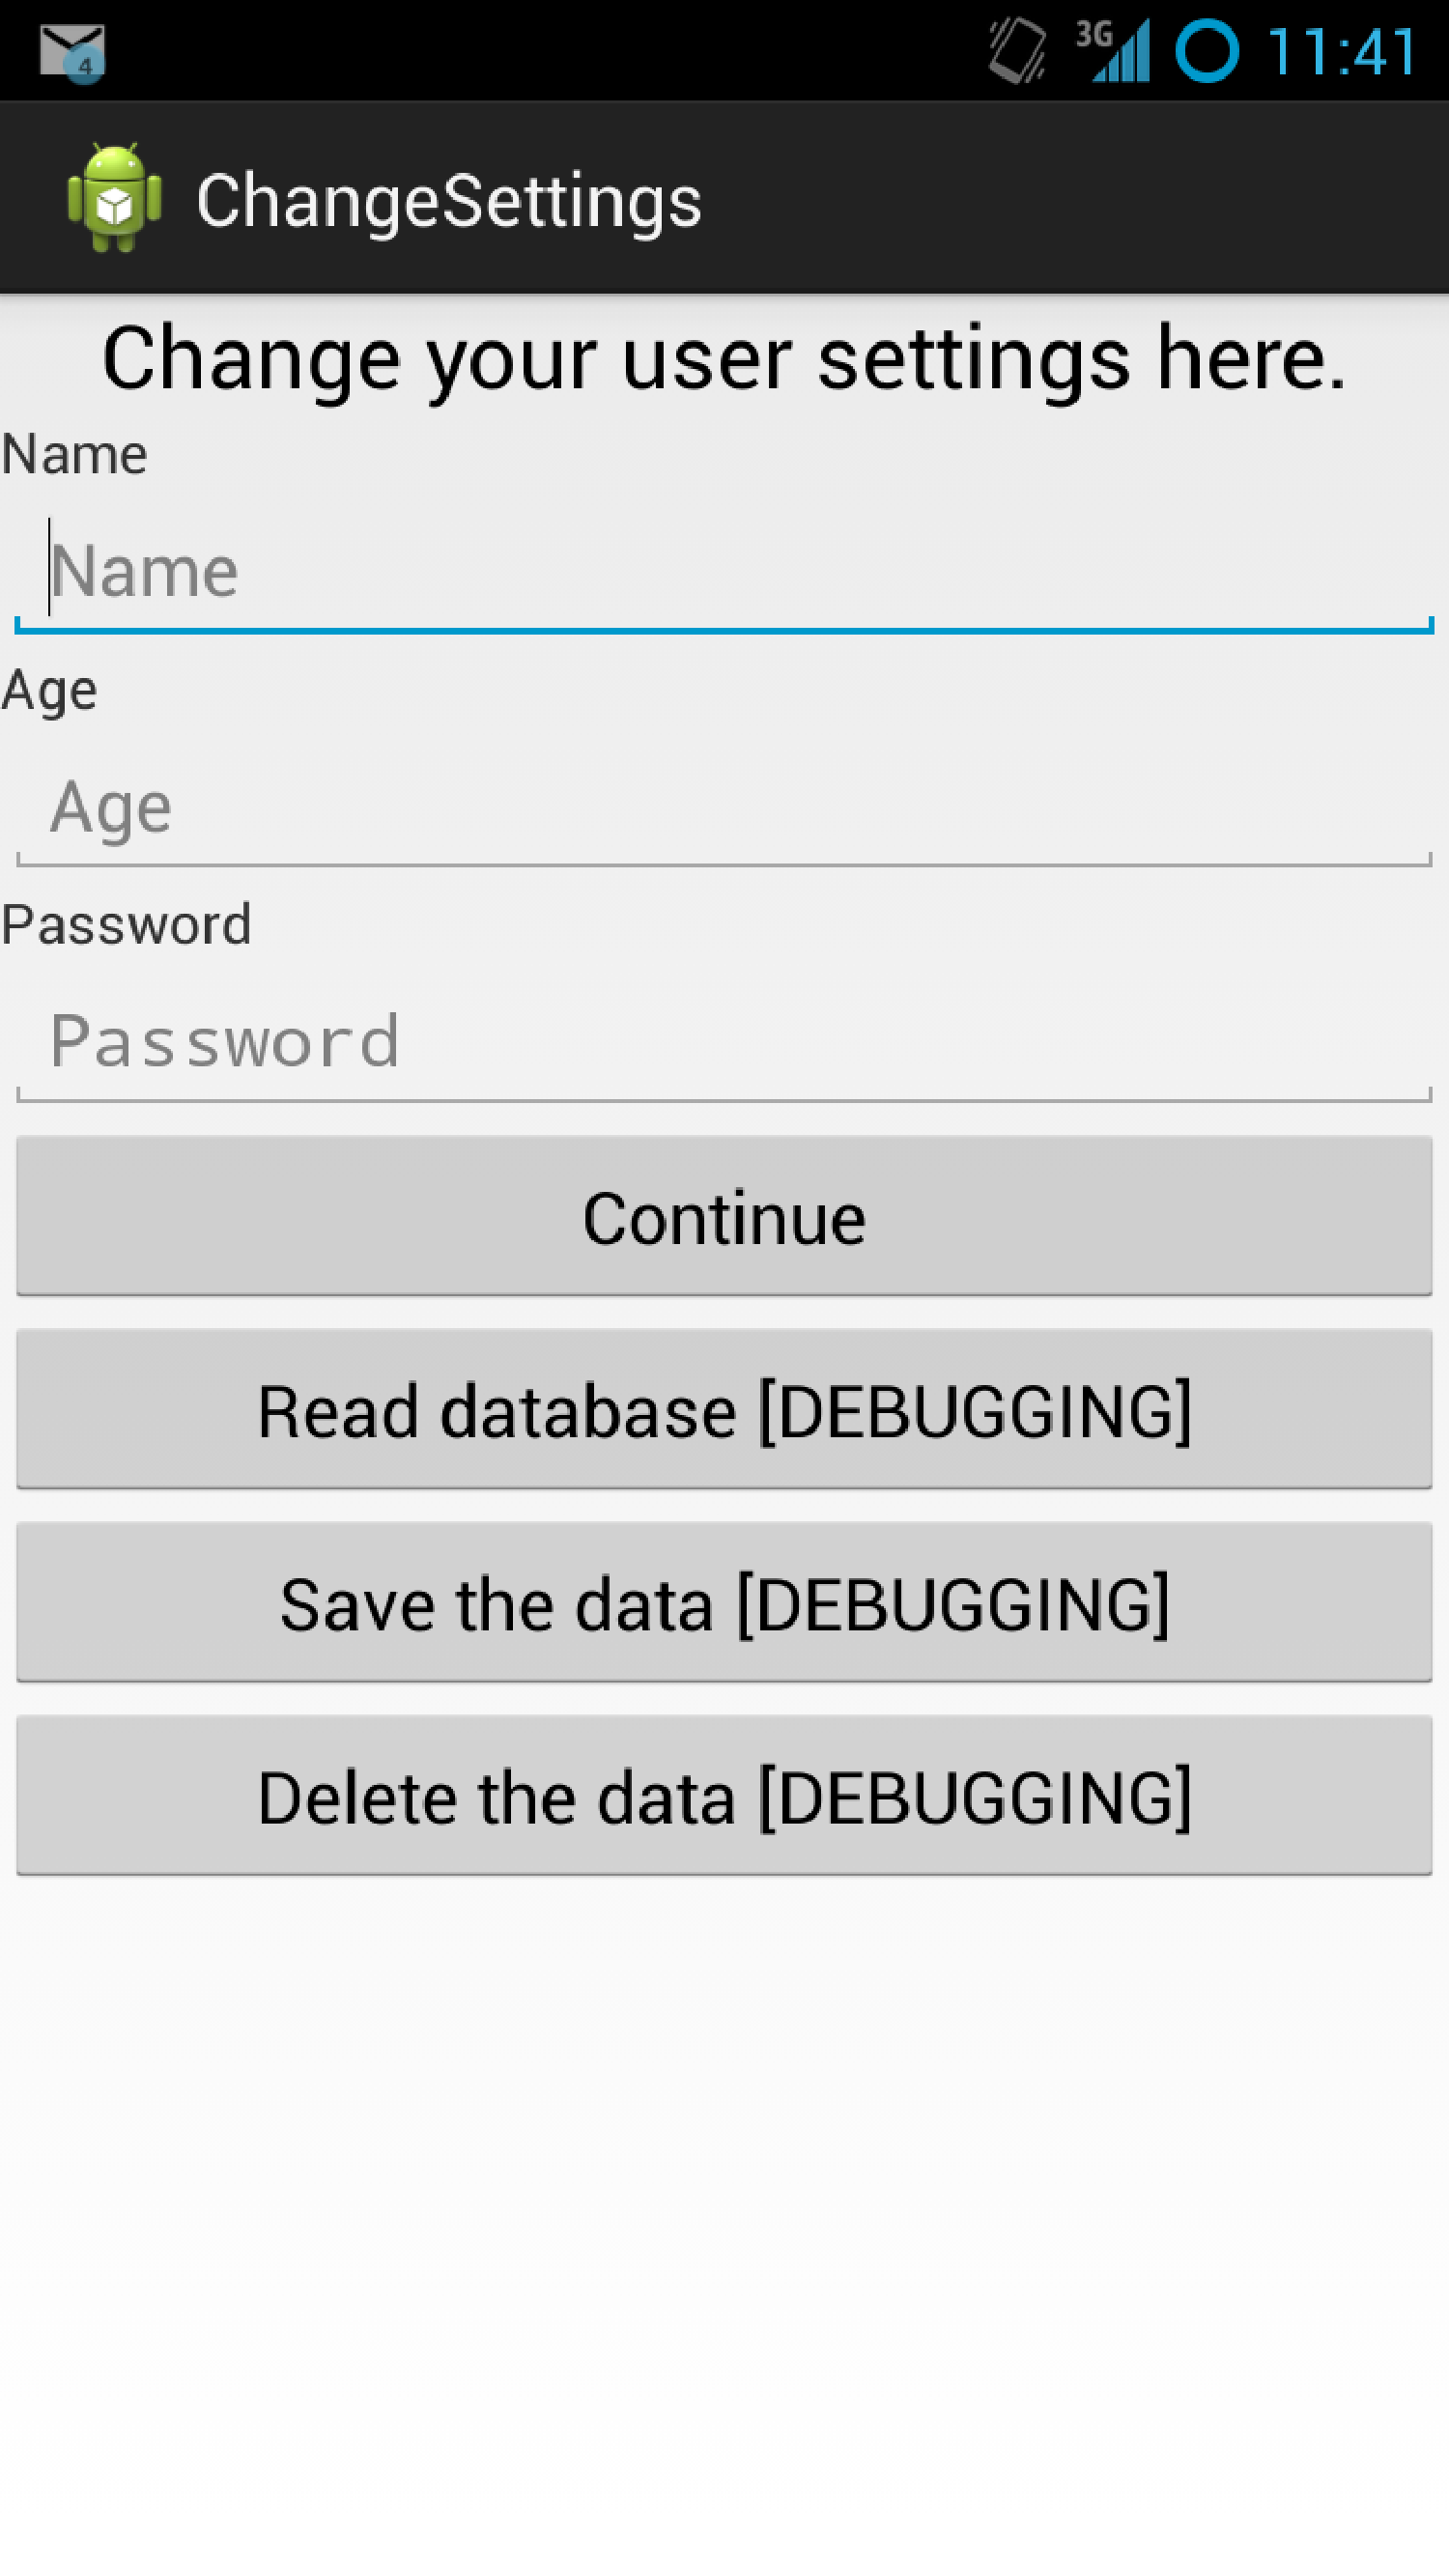
\includegraphics[clip = true, trim = 0 320 0 60,
 scale=0.2]{change_settings}
 \caption{A screenshot of the app's change settings activity}
 \label{fig:change-settings-screenshot}
\end{figure}

When the app enters this activity, it prompts the user to enter his user
name and password. When the user presses the `continue button', the old database
entry and app-wide variable is overwritten with the new values the user entered.

\subsection{Main Activity}

The main activity is the activity which is responsible for encrypting and
sending the purchase requests to the web server, receiving and decrypting
the purchase approval codes and sending the NFC messages to the vending machines
NFC receiver. See Figure \ref{fig:main-activity} for a process flow diagram
and Figure \ref{fig:main-activity-screenshot} for a screenshot of this activity.

\begin{figure}
 \centering 
 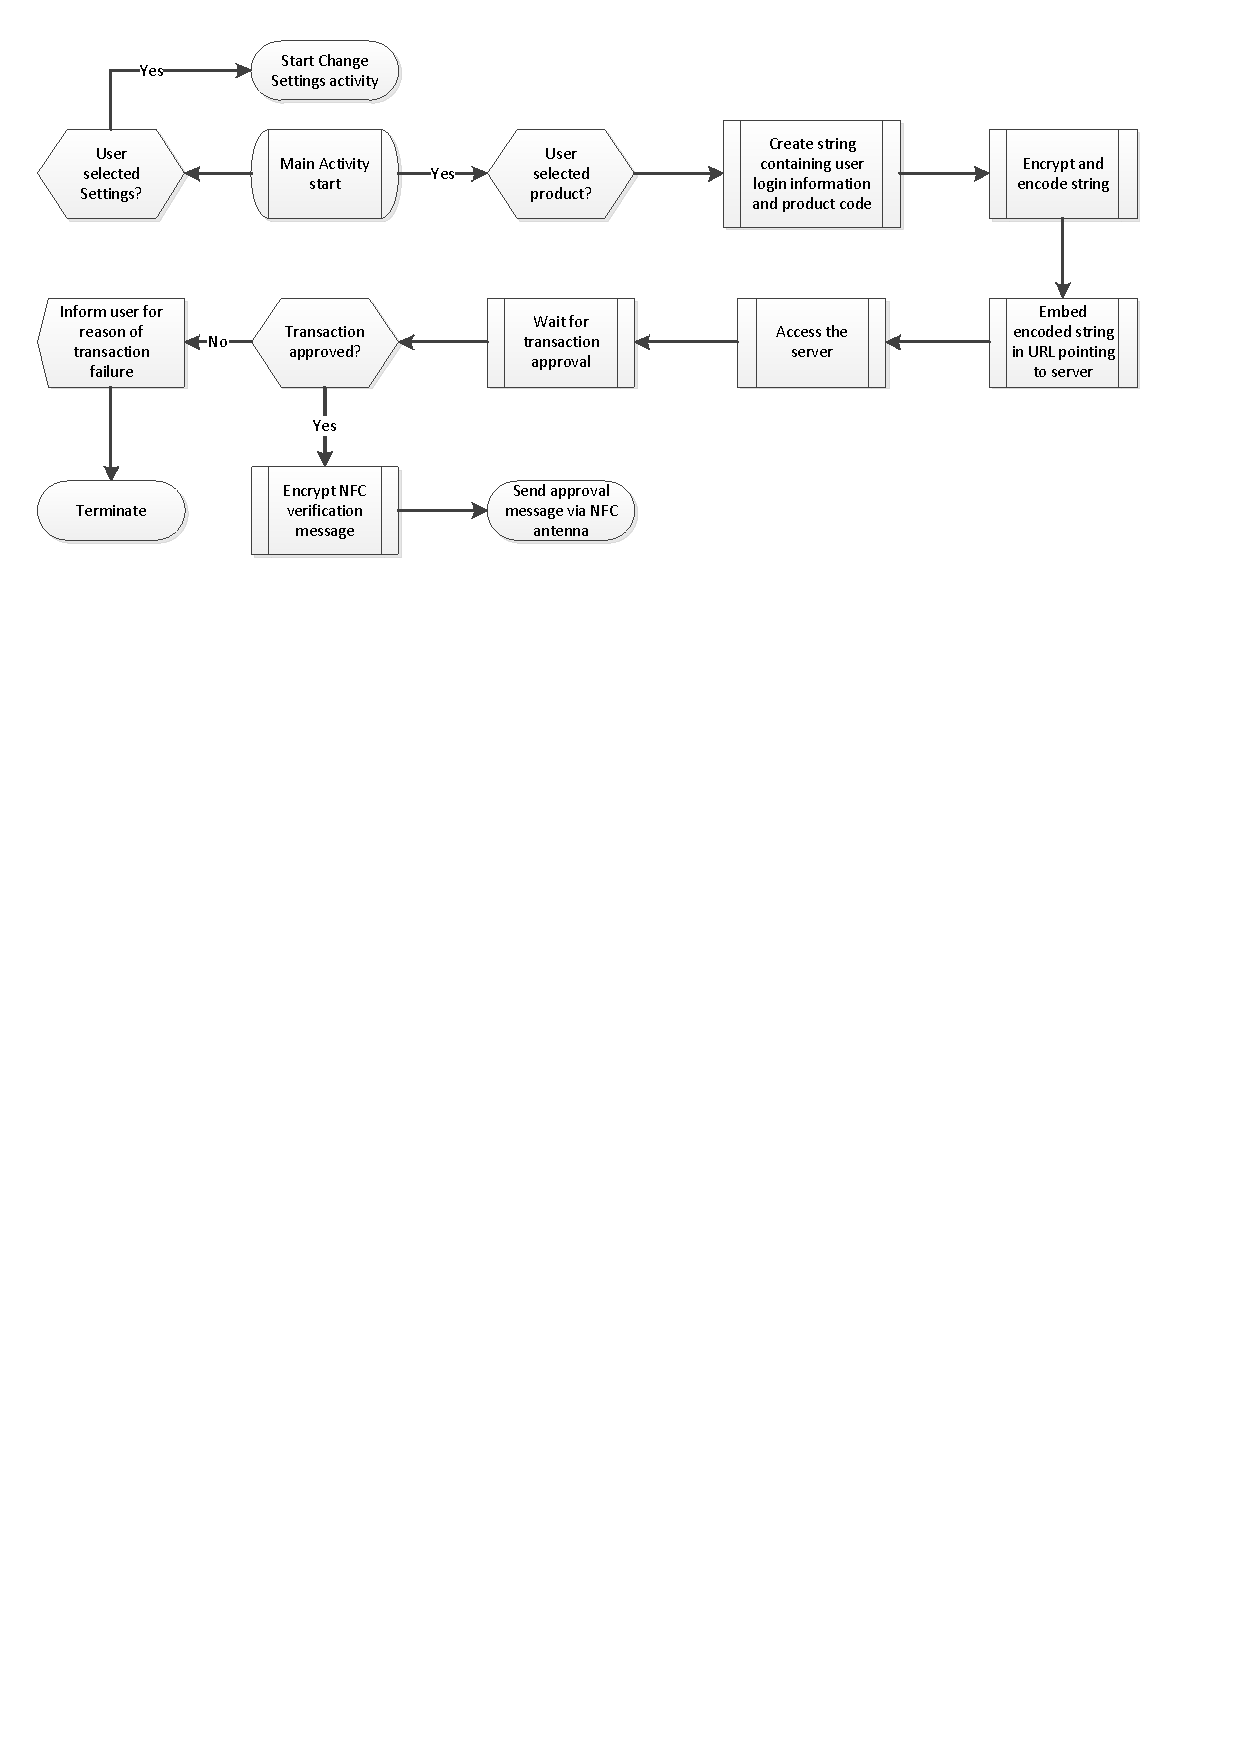
\includegraphics[clip = true, trim = 0 570 0 20,
 scale=0.7]{app_main_processflow}
 \caption{The process flow of the Main activity}
 \label{fig:main-activity}
\end{figure}

\begin{figure}
 \centering 
 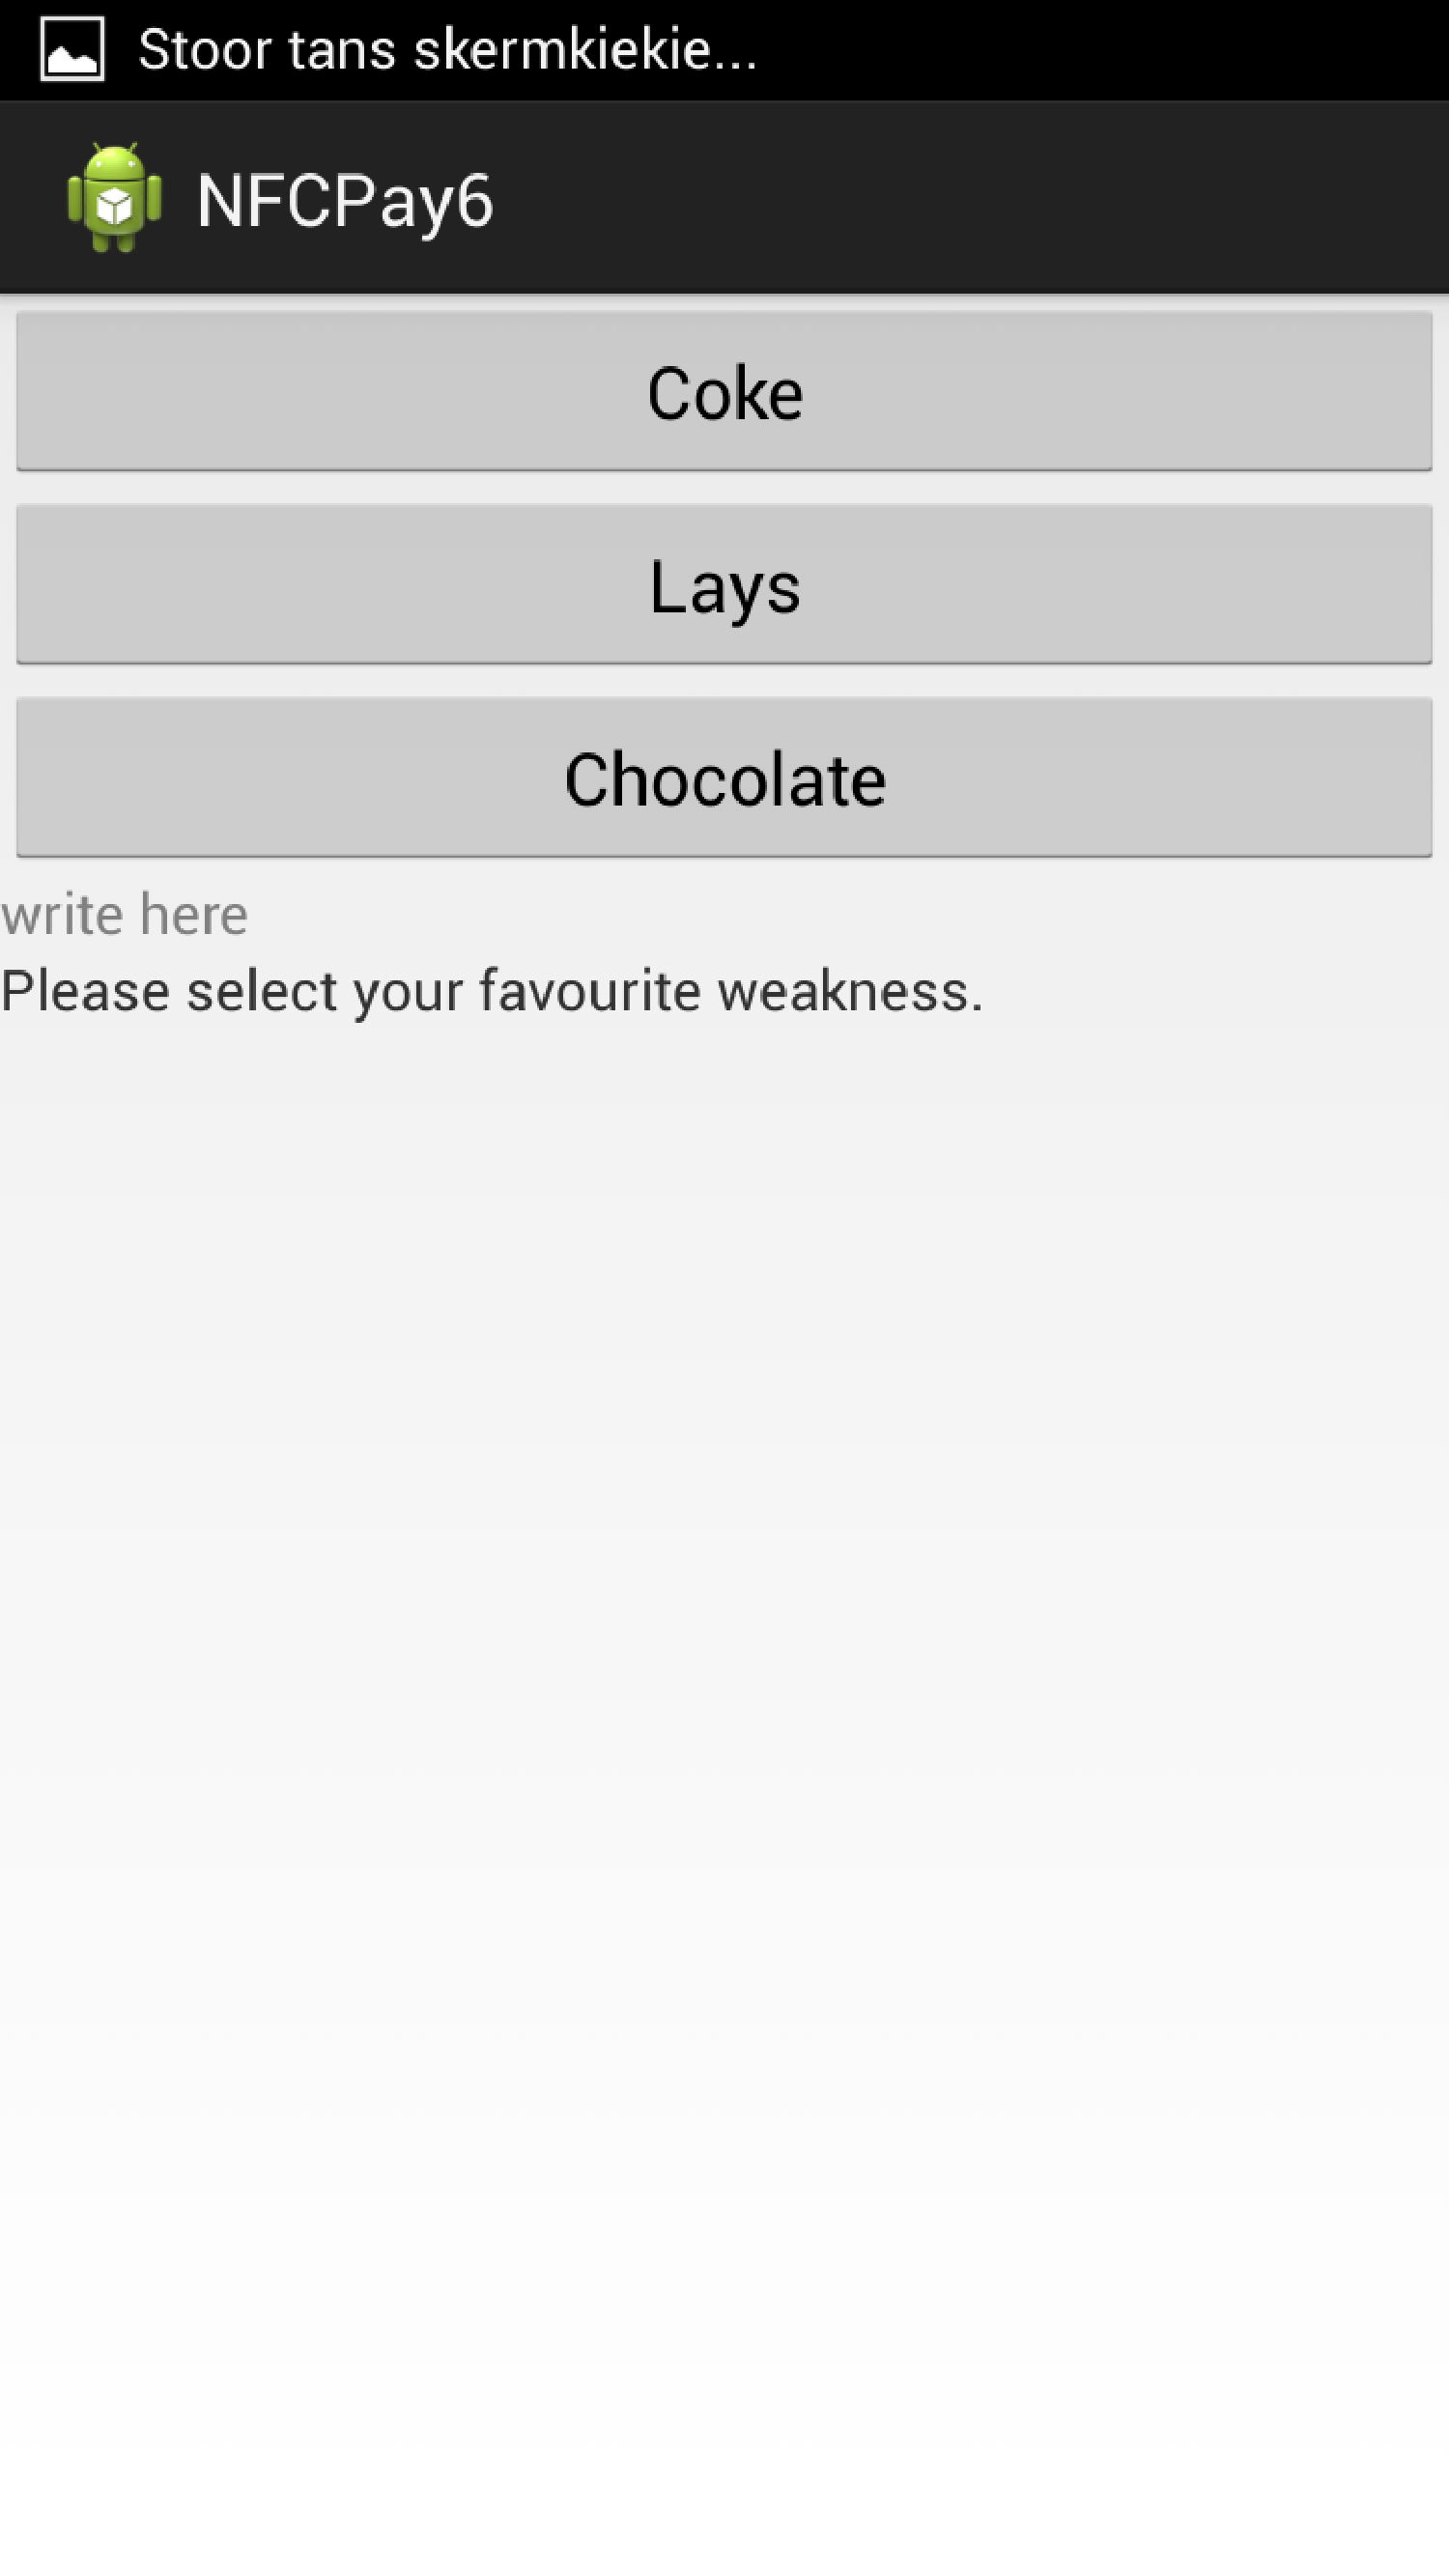
\includegraphics[clip = true, trim = 0 520 0 60,
 scale=0.2]{main_menu}
 \caption{A screenshot of the app's main activity activity}
 \label{fig:main-activity-screenshot}
\end{figure}

As seen from Figure \ref{fig:main-activity-screenshot}, the activity presents
the user with a list of products. When the user selects a product to buy, the
activity forms a data string by adding the product code, the user's login
name and password together. This data string is then encrypted with the
server's public key half and then encoded with base 64. This encoded string
is then embedded into a Uniform Resource Locator (URL) which points to the
web server. 

The activity then goes to this URL in the background which prompts the server to
process the transaction (see Section \ref{sec:app-nfc} for more details on the
server's NFC processes). The server then tells the activity if the transaction
has been approved or denied. If it has been denied, the user is informed what was wrong. 

If it is approved, the activity activates the cellphone's NFC antennae which
transmits an encrypted approval message to the vending machine's NFC receiver. 
